\documentclass[11pt]{article}
\usepackage[textwidth=18.0cm, textheight=23.0cm, top=2.0cm]{geometry}
\usepackage{pst-all}
\usepackage{amssymb}
\usepackage{tikz}
\usepackage{underscore}\begin{document}
\pagestyle{empty}


ClassName: \underline{\textbf{Class_08.2bp-42}}
\par
BinSize: \underline{\textbf{100 × 100}}
\par
ReduceSize: \underline{\textbf{100 × 100}}
\par
TypeNum: \underline{\textbf{99}}
\par
Num: \underline{\textbf{100}}
\par
OutS: \underline{\textbf{240000}}
\par
InS: \underline{\textbf{206333}}
\par
Rate: \underline{\textbf{0.860}}
\par
UB: \underline{\textbf{24}}
\par
LB0: \underline{\textbf{24}}
\par
LB: \underline{\textbf{24}}
\par
LBWithCut: \underline{\textbf{24}}
\par
NodeCut: \underline{\textbf{0}}
\par
ExtendedNodeCnt: \underline{\textbf{1}}
\par
GenNodeCnt: \underline{\textbf{1}}
\par
PrimalNode: \underline{\textbf{0}}
\par
ColumnCount: \underline{\textbf{24}}
\par
TotalCutCount: \underline{\textbf{0}}
\par
RootCutCount: \underline{\textbf{0}}
\par
LPSolverCnt: \underline{\textbf{1}}
\par
PricingSolverCnt: \underline{\textbf{0}}
\par
BranchAndBoundNum: \underline{\textbf{1}}
\par
isOpt: \underline{\textbf{true}}
\par
TimeOnInitSolution: \underline{\textbf{0.330 s}}
\par
TimeOnPrimal: \underline{\textbf{0.000 s}}
\par
TimeOnPricing: \underline{\textbf{0.000 s}}
\par
TimeOnRmp: \underline{\textbf{0.062 s}}
\par
TotalTime: \underline{\textbf{0.470 s}}
\par
\newpage


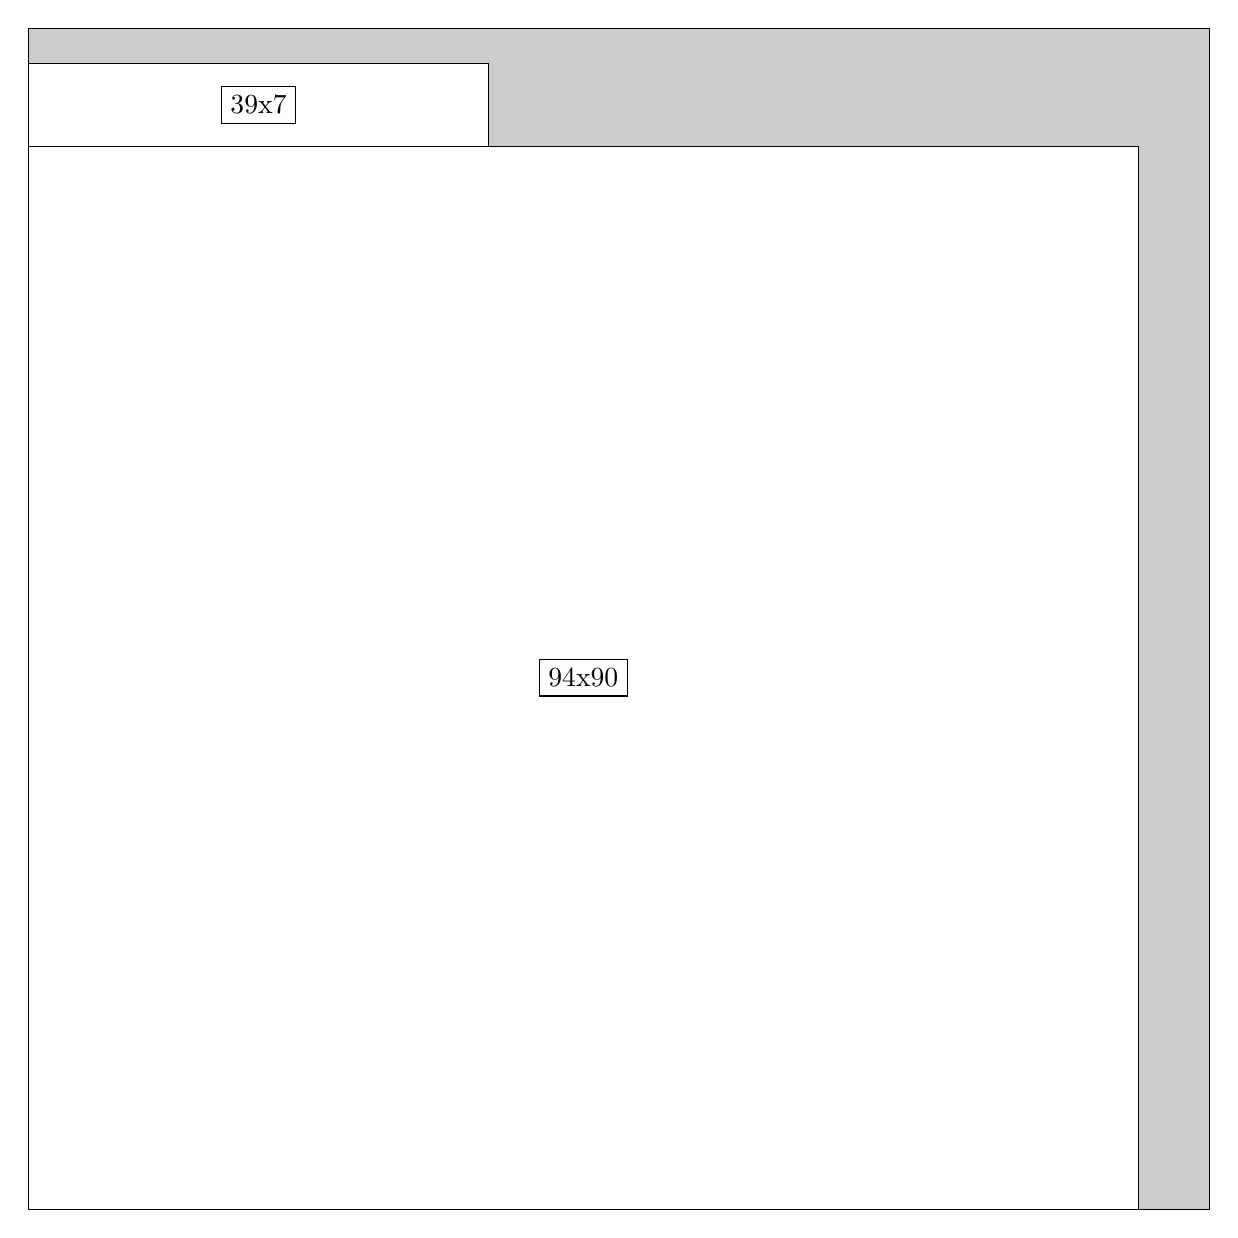
\begin{tikzpicture}[shorten >=1pt,scale=1.0,every node/.style={scale=1.0},->]
\tikzstyle{vertex}=[circle,fill=black!25,minimum size=14pt,inner sep=0pt]
\filldraw[fill=gray!40!white, draw=black] (0,0) rectangle (15.0,15.0);
\foreach \name/\x/\y/\w/\h in {94x90/0.0/0.0/14.1/13.5,39x7/0.0/13.5/5.85/1.05}
\filldraw[fill=white!40!white, draw=black] (\x,\y) rectangle node[draw] (\name) {\name} ++(\w,\h);
\end{tikzpicture}


w =94 , h =90 , x =0 , y =0 , v =8460
\par
w =39 , h =7 , x =0 , y =90 , v =273
\par
\newpage


\begin{tikzpicture}[shorten >=1pt,scale=1.0,every node/.style={scale=1.0},->]
\tikzstyle{vertex}=[circle,fill=black!25,minimum size=14pt,inner sep=0pt]
\filldraw[fill=gray!40!white, draw=black] (0,0) rectangle (15.0,15.0);
\foreach \name/\x/\y/\w/\h in {87x93/0.0/0.0/13.049999999999999/13.95,13x94/13.049999999999999/0.0/1.95/14.1,79x7/0.0/13.95/11.85/1.05}
\filldraw[fill=white!40!white, draw=black] (\x,\y) rectangle node[draw] (\name) {\name} ++(\w,\h);
\end{tikzpicture}


w =87 , h =93 , x =0 , y =0 , v =8091
\par
w =13 , h =94 , x =87 , y =0 , v =1222
\par
w =79 , h =7 , x =0 , y =93 , v =553
\par
\newpage


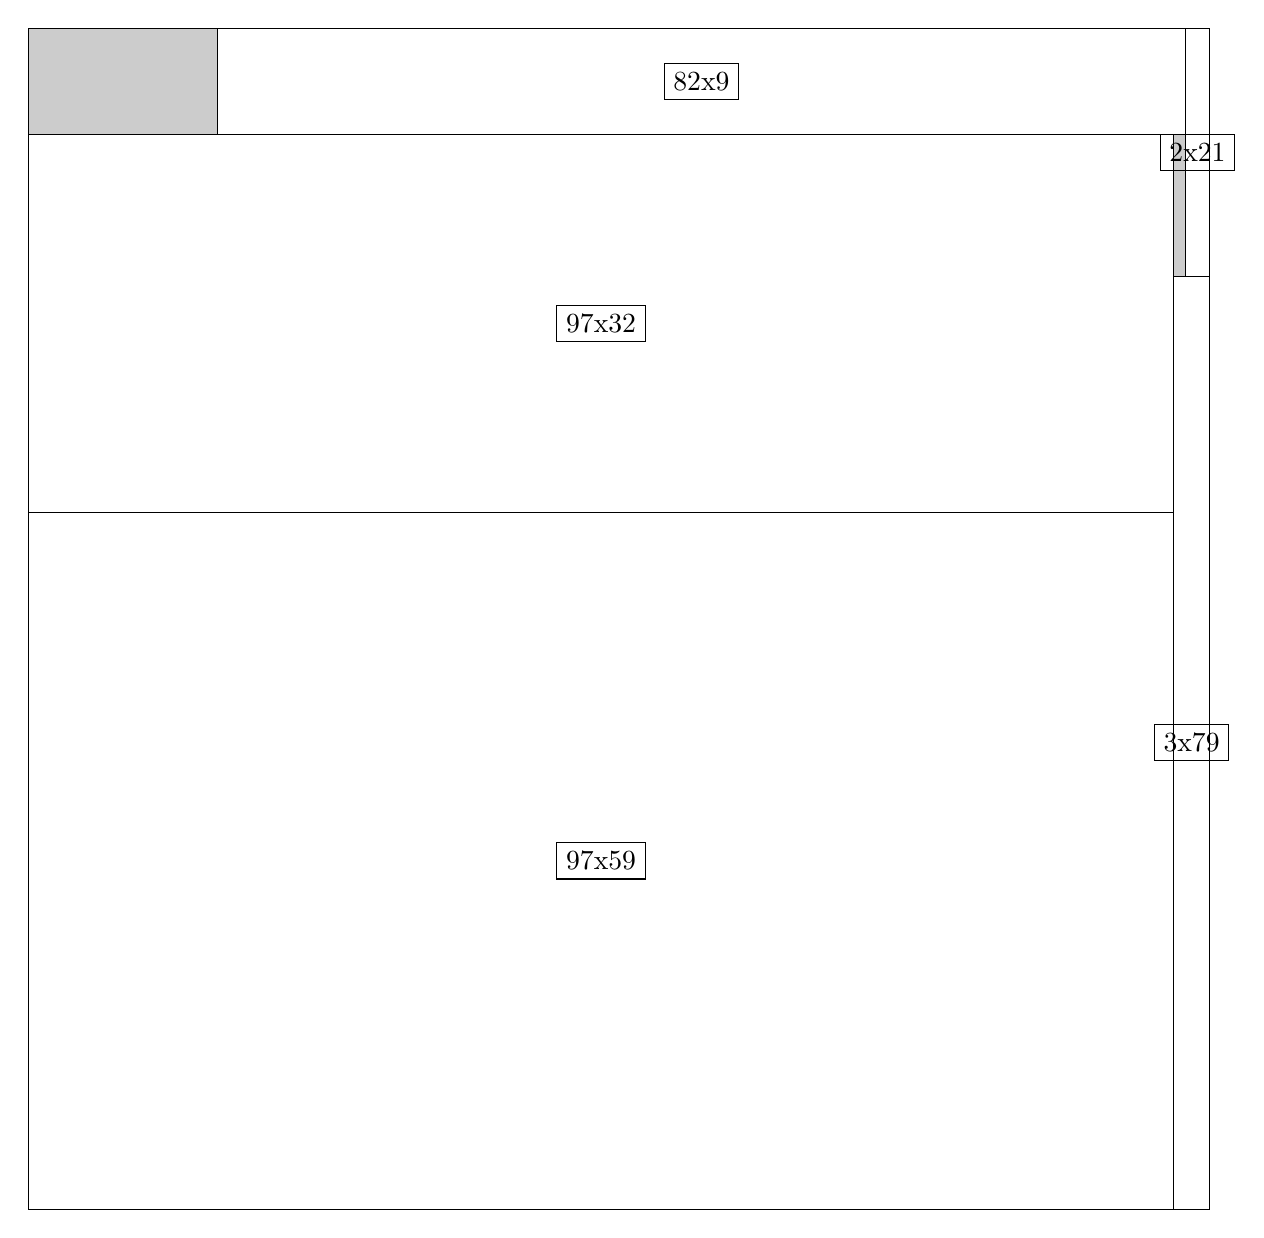
\begin{tikzpicture}[shorten >=1pt,scale=1.0,every node/.style={scale=1.0},->]
\tikzstyle{vertex}=[circle,fill=black!25,minimum size=14pt,inner sep=0pt]
\filldraw[fill=gray!40!white, draw=black] (0,0) rectangle (15.0,15.0);
\foreach \name/\x/\y/\w/\h in {97x59/0.0/0.0/14.549999999999999/8.85,97x32/0.0/8.85/14.549999999999999/4.8,82x9/2.4/13.65/12.299999999999999/1.3499999999999999,3x79/14.549999999999999/0.0/0.44999999999999996/11.85,2x21/14.7/11.85/0.3/3.15}
\filldraw[fill=white!40!white, draw=black] (\x,\y) rectangle node[draw] (\name) {\name} ++(\w,\h);
\end{tikzpicture}


w =97 , h =59 , x =0 , y =0 , v =5723
\par
w =97 , h =32 , x =0 , y =59 , v =3104
\par
w =82 , h =9 , x =16 , y =91 , v =738
\par
w =3 , h =79 , x =97 , y =0 , v =237
\par
w =2 , h =21 , x =98 , y =79 , v =42
\par
\newpage


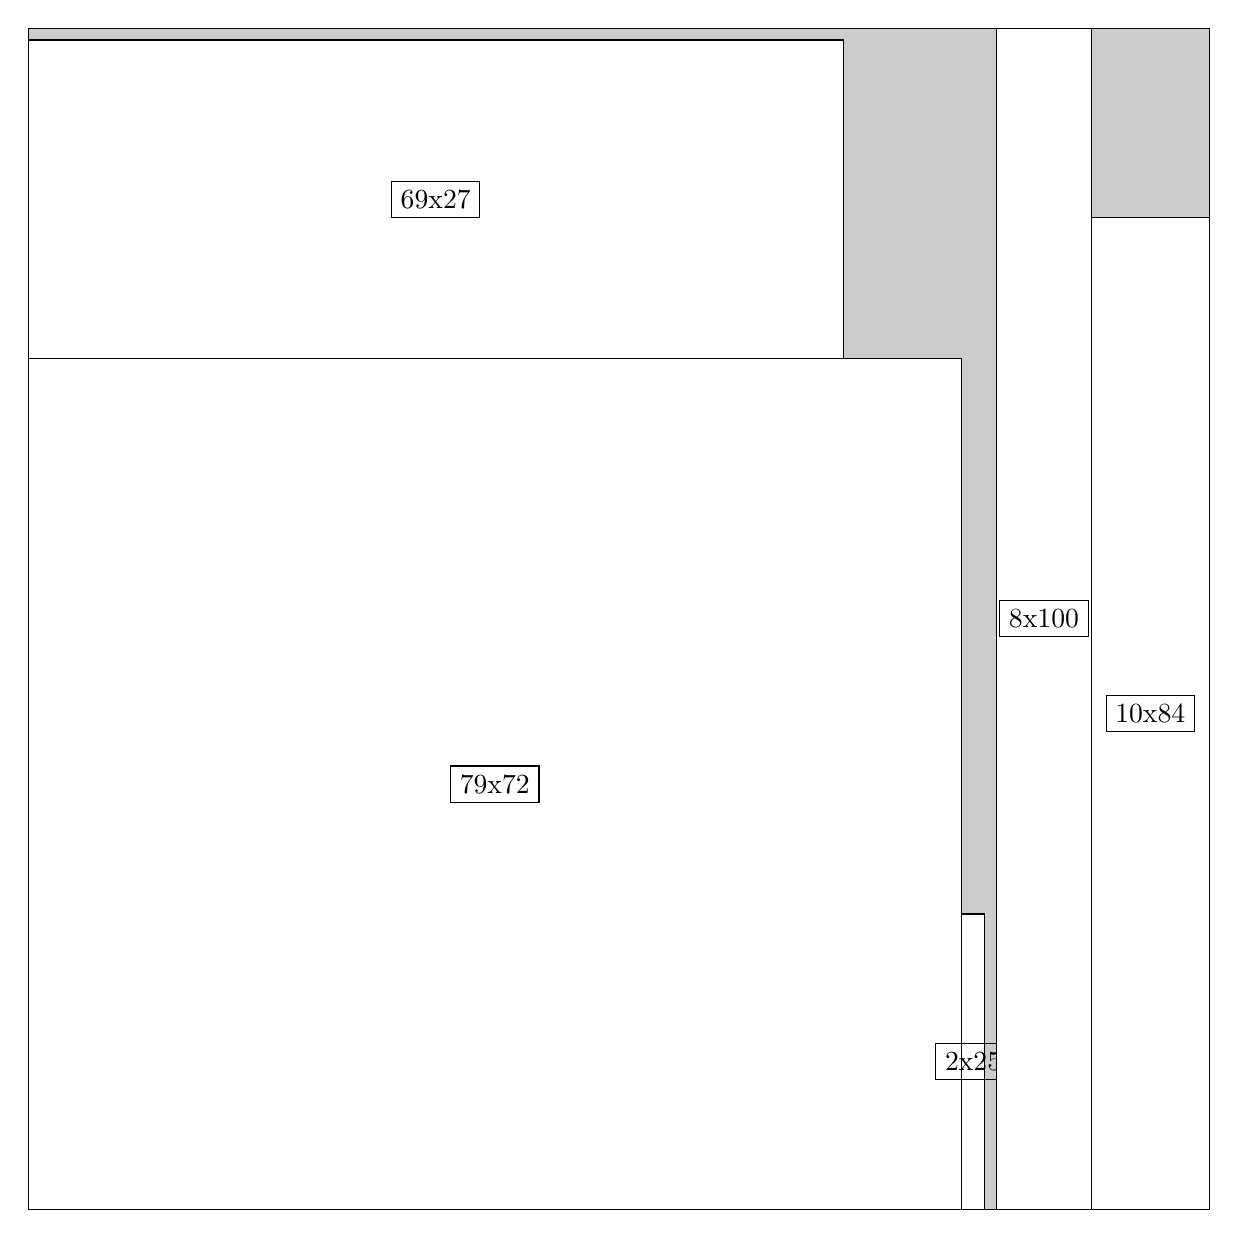
\begin{tikzpicture}[shorten >=1pt,scale=1.0,every node/.style={scale=1.0},->]
\tikzstyle{vertex}=[circle,fill=black!25,minimum size=14pt,inner sep=0pt]
\filldraw[fill=gray!40!white, draw=black] (0,0) rectangle (15.0,15.0);
\foreach \name/\x/\y/\w/\h in {79x72/0.0/0.0/11.85/10.799999999999999,2x25/11.85/0.0/0.3/3.75,69x27/0.0/10.799999999999999/10.35/4.05,10x84/13.5/0.0/1.5/12.6,8x100/12.299999999999999/0.0/1.2/15.0}
\filldraw[fill=white!40!white, draw=black] (\x,\y) rectangle node[draw] (\name) {\name} ++(\w,\h);
\end{tikzpicture}


w =79 , h =72 , x =0 , y =0 , v =5688
\par
w =2 , h =25 , x =79 , y =0 , v =50
\par
w =69 , h =27 , x =0 , y =72 , v =1863
\par
w =10 , h =84 , x =90 , y =0 , v =840
\par
w =8 , h =100 , x =82 , y =0 , v =800
\par
\newpage


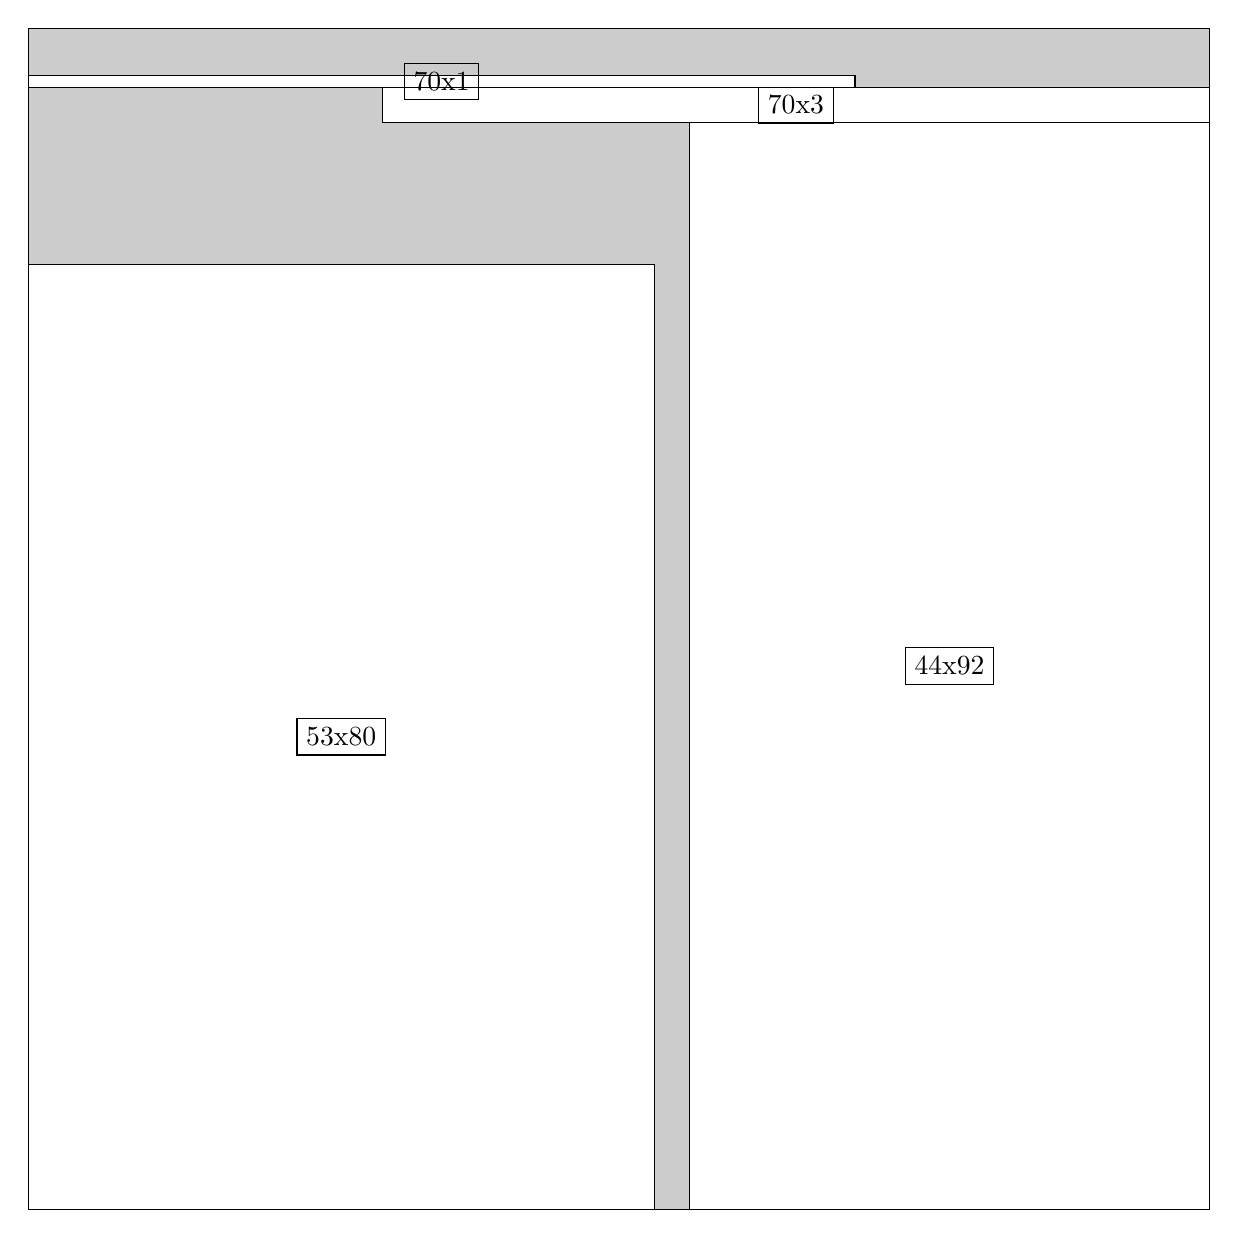
\begin{tikzpicture}[shorten >=1pt,scale=1.0,every node/.style={scale=1.0},->]
\tikzstyle{vertex}=[circle,fill=black!25,minimum size=14pt,inner sep=0pt]
\filldraw[fill=gray!40!white, draw=black] (0,0) rectangle (15.0,15.0);
\foreach \name/\x/\y/\w/\h in {53x80/0.0/0.0/7.949999999999999/12.0,44x92/8.4/0.0/6.6/13.799999999999999,70x3/4.5/13.799999999999999/10.5/0.44999999999999996,70x1/0.0/14.25/10.5/0.15}
\filldraw[fill=white!40!white, draw=black] (\x,\y) rectangle node[draw] (\name) {\name} ++(\w,\h);
\end{tikzpicture}


w =53 , h =80 , x =0 , y =0 , v =4240
\par
w =44 , h =92 , x =56 , y =0 , v =4048
\par
w =70 , h =3 , x =30 , y =92 , v =210
\par
w =70 , h =1 , x =0 , y =95 , v =70
\par
\newpage


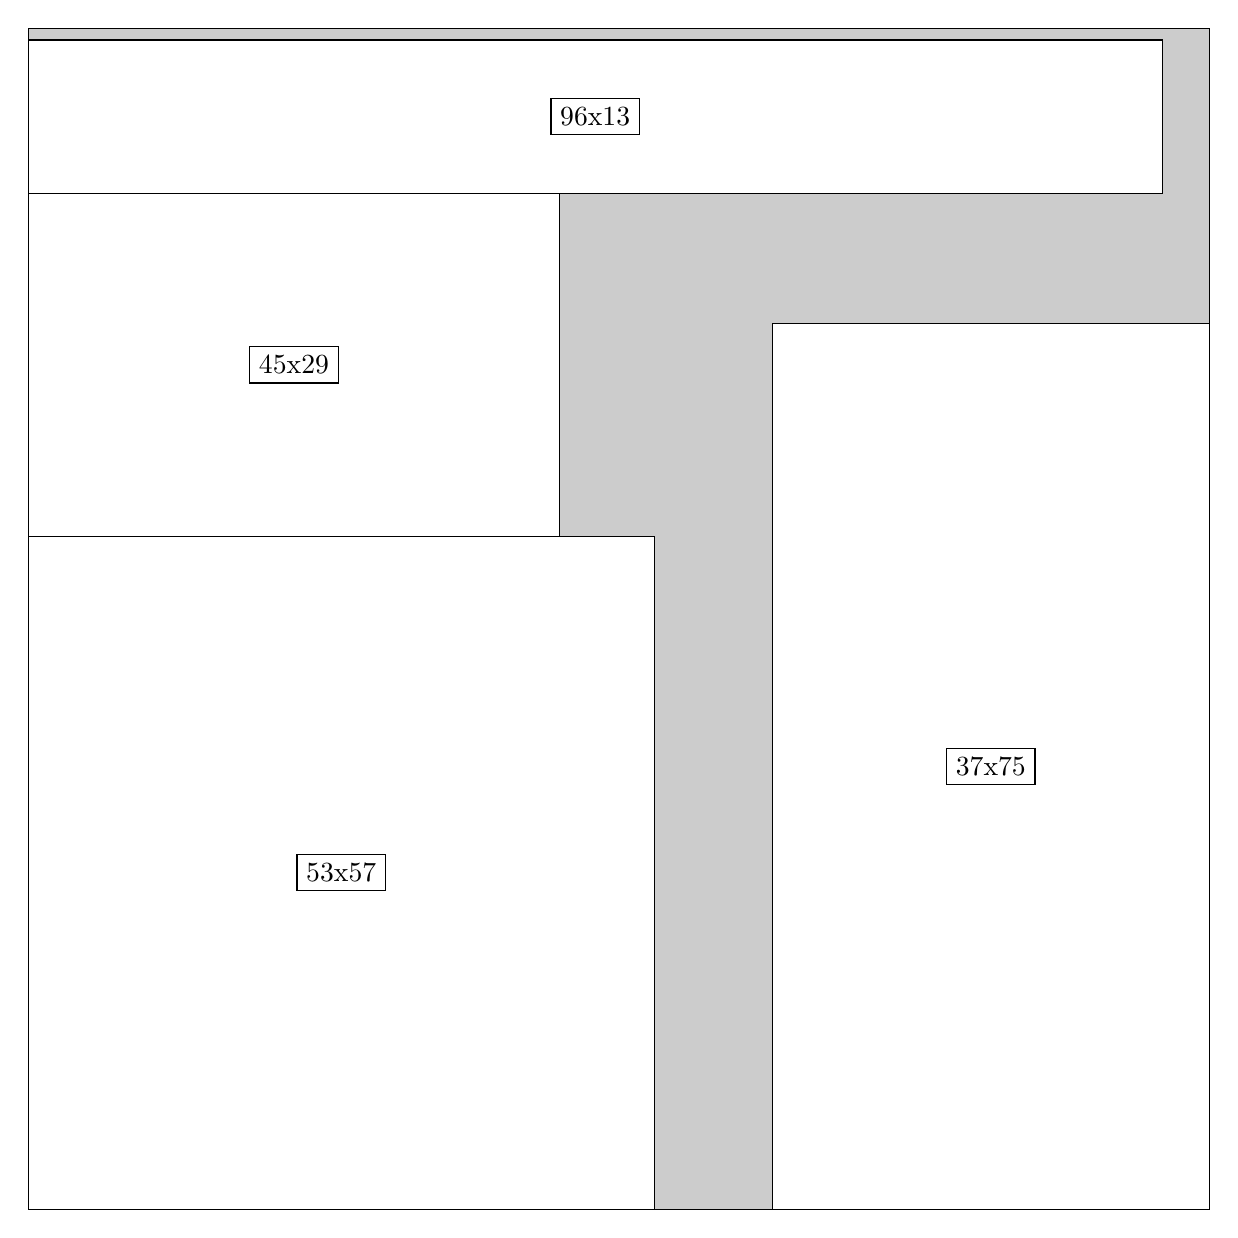
\begin{tikzpicture}[shorten >=1pt,scale=1.0,every node/.style={scale=1.0},->]
\tikzstyle{vertex}=[circle,fill=black!25,minimum size=14pt,inner sep=0pt]
\filldraw[fill=gray!40!white, draw=black] (0,0) rectangle (15.0,15.0);
\foreach \name/\x/\y/\w/\h in {53x57/0.0/0.0/7.949999999999999/8.549999999999999,37x75/9.45/0.0/5.55/11.25,45x29/0.0/8.549999999999999/6.75/4.35,96x13/0.0/12.9/14.399999999999999/1.95}
\filldraw[fill=white!40!white, draw=black] (\x,\y) rectangle node[draw] (\name) {\name} ++(\w,\h);
\end{tikzpicture}


w =53 , h =57 , x =0 , y =0 , v =3021
\par
w =37 , h =75 , x =63 , y =0 , v =2775
\par
w =45 , h =29 , x =0 , y =57 , v =1305
\par
w =96 , h =13 , x =0 , y =86 , v =1248
\par
\newpage


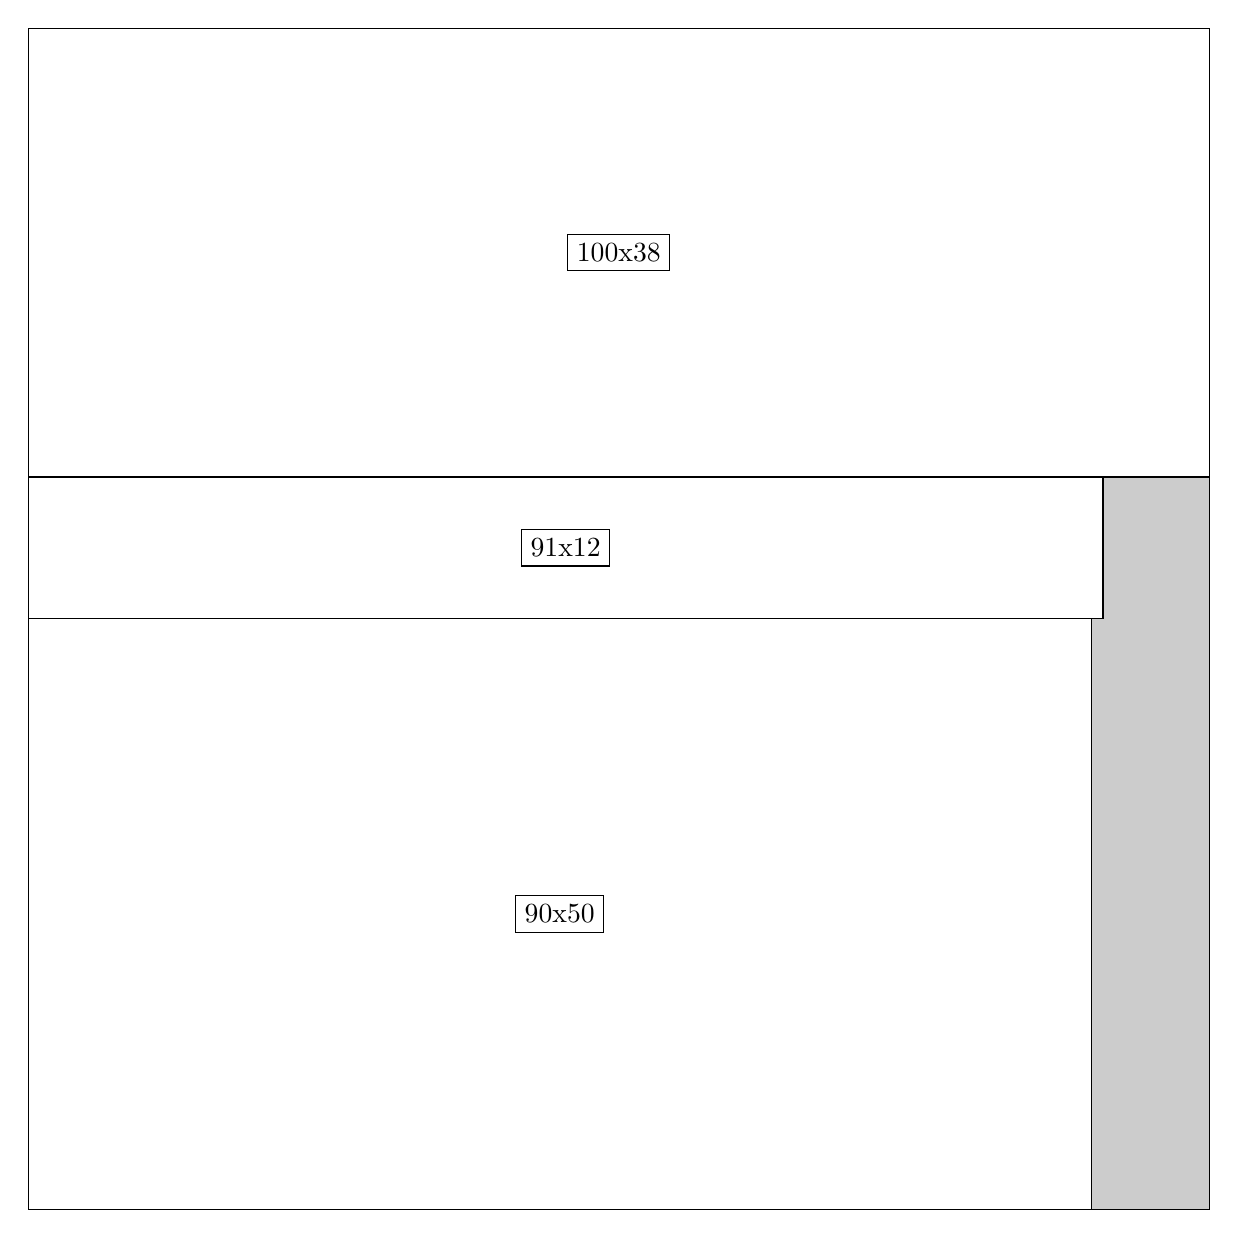
\begin{tikzpicture}[shorten >=1pt,scale=1.0,every node/.style={scale=1.0},->]
\tikzstyle{vertex}=[circle,fill=black!25,minimum size=14pt,inner sep=0pt]
\filldraw[fill=gray!40!white, draw=black] (0,0) rectangle (15.0,15.0);
\foreach \name/\x/\y/\w/\h in {90x50/0.0/0.0/13.5/7.5,100x38/0.0/9.299999999999999/15.0/5.7,91x12/0.0/7.5/13.65/1.7999999999999998}
\filldraw[fill=white!40!white, draw=black] (\x,\y) rectangle node[draw] (\name) {\name} ++(\w,\h);
\end{tikzpicture}


w =90 , h =50 , x =0 , y =0 , v =4500
\par
w =100 , h =38 , x =0 , y =62 , v =3800
\par
w =91 , h =12 , x =0 , y =50 , v =1092
\par
\newpage


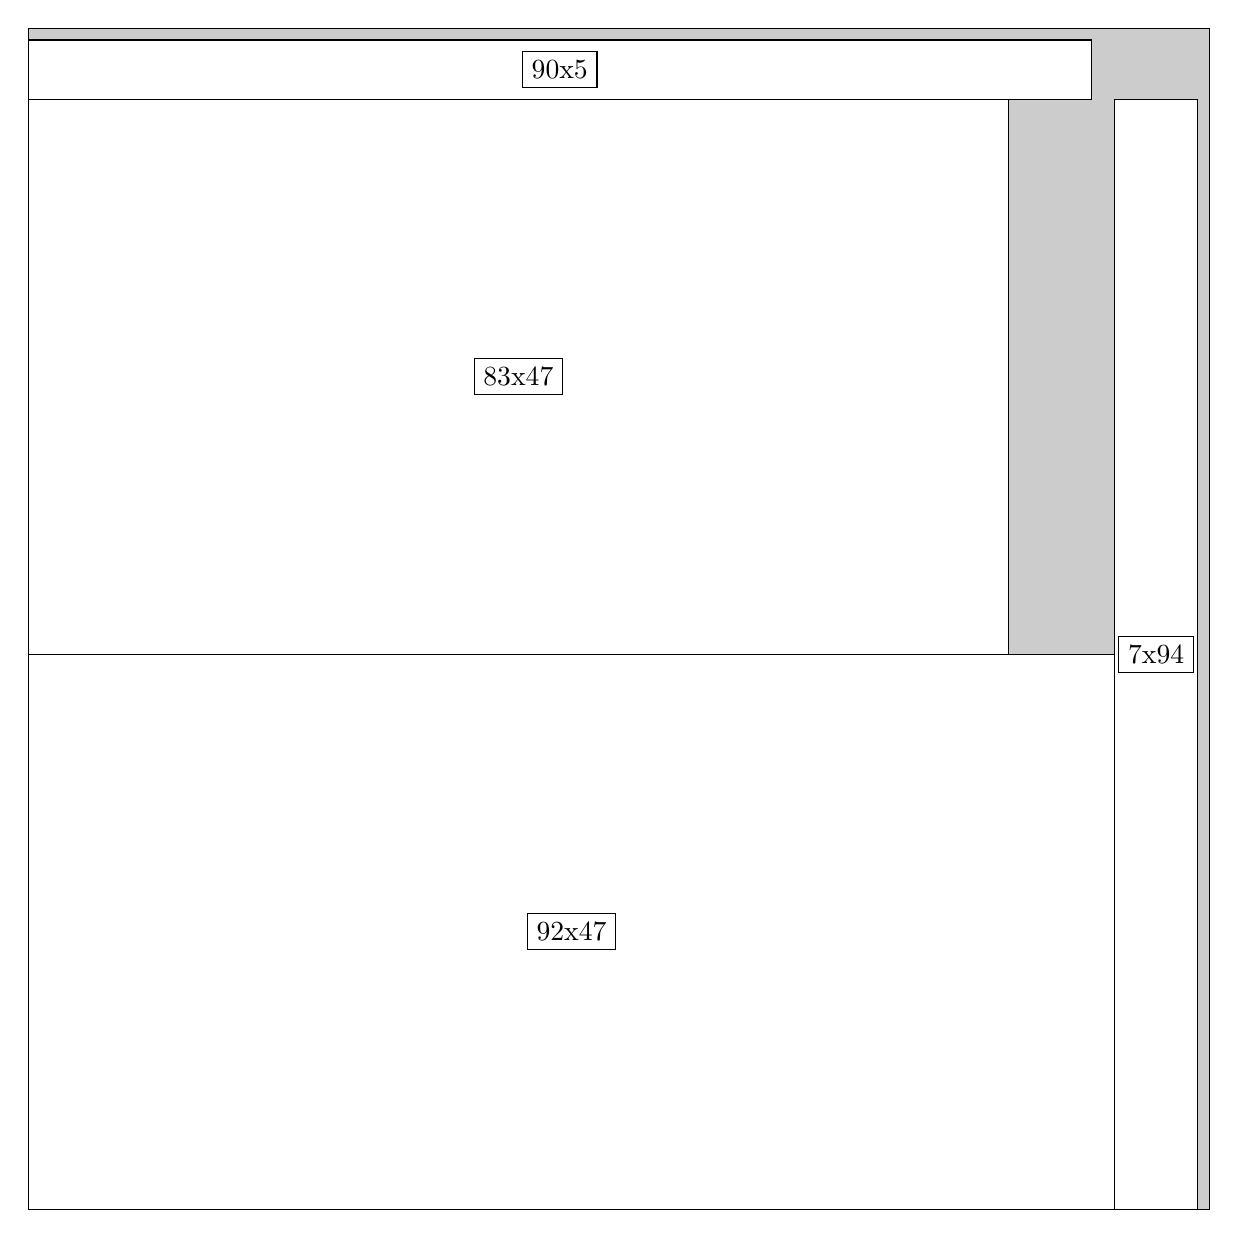
\begin{tikzpicture}[shorten >=1pt,scale=1.0,every node/.style={scale=1.0},->]
\tikzstyle{vertex}=[circle,fill=black!25,minimum size=14pt,inner sep=0pt]
\filldraw[fill=gray!40!white, draw=black] (0,0) rectangle (15.0,15.0);
\foreach \name/\x/\y/\w/\h in {92x47/0.0/0.0/13.799999999999999/7.05,83x47/0.0/7.05/12.45/7.05,7x94/13.799999999999999/0.0/1.05/14.1,90x5/0.0/14.1/13.5/0.75}
\filldraw[fill=white!40!white, draw=black] (\x,\y) rectangle node[draw] (\name) {\name} ++(\w,\h);
\end{tikzpicture}


w =92 , h =47 , x =0 , y =0 , v =4324
\par
w =83 , h =47 , x =0 , y =47 , v =3901
\par
w =7 , h =94 , x =92 , y =0 , v =658
\par
w =90 , h =5 , x =0 , y =94 , v =450
\par
\newpage


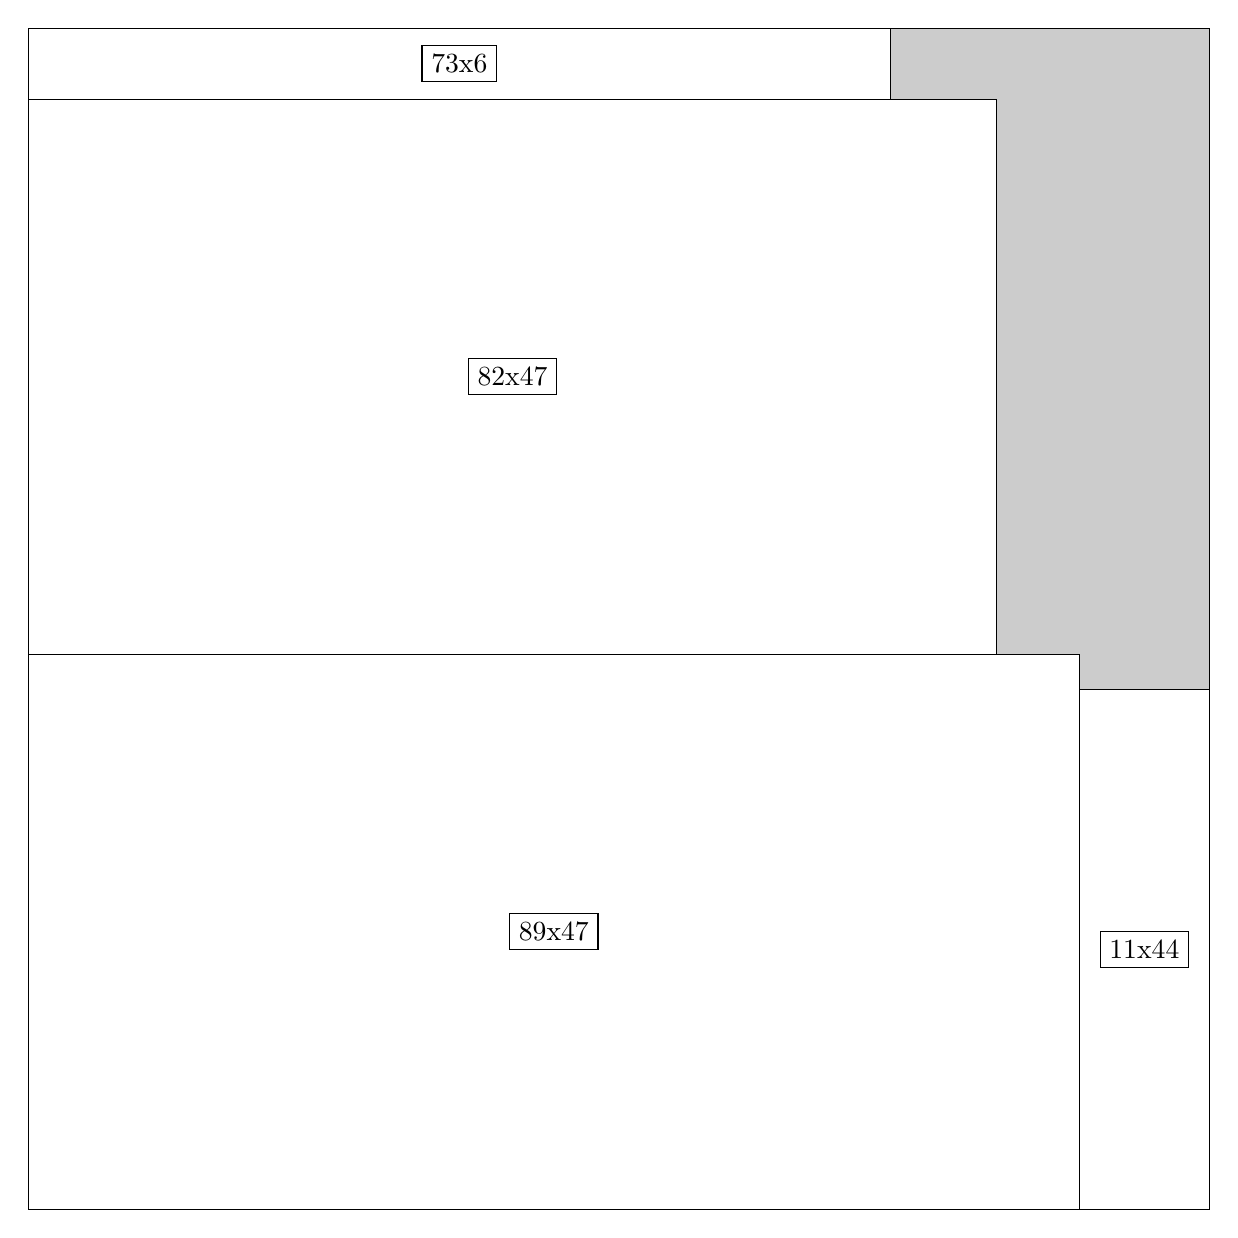
\begin{tikzpicture}[shorten >=1pt,scale=1.0,every node/.style={scale=1.0},->]
\tikzstyle{vertex}=[circle,fill=black!25,minimum size=14pt,inner sep=0pt]
\filldraw[fill=gray!40!white, draw=black] (0,0) rectangle (15.0,15.0);
\foreach \name/\x/\y/\w/\h in {89x47/0.0/0.0/13.35/7.05,82x47/0.0/7.05/12.299999999999999/7.05,11x44/13.35/0.0/1.65/6.6,73x6/0.0/14.1/10.95/0.8999999999999999}
\filldraw[fill=white!40!white, draw=black] (\x,\y) rectangle node[draw] (\name) {\name} ++(\w,\h);
\end{tikzpicture}


w =89 , h =47 , x =0 , y =0 , v =4183
\par
w =82 , h =47 , x =0 , y =47 , v =3854
\par
w =11 , h =44 , x =89 , y =0 , v =484
\par
w =73 , h =6 , x =0 , y =94 , v =438
\par
\newpage


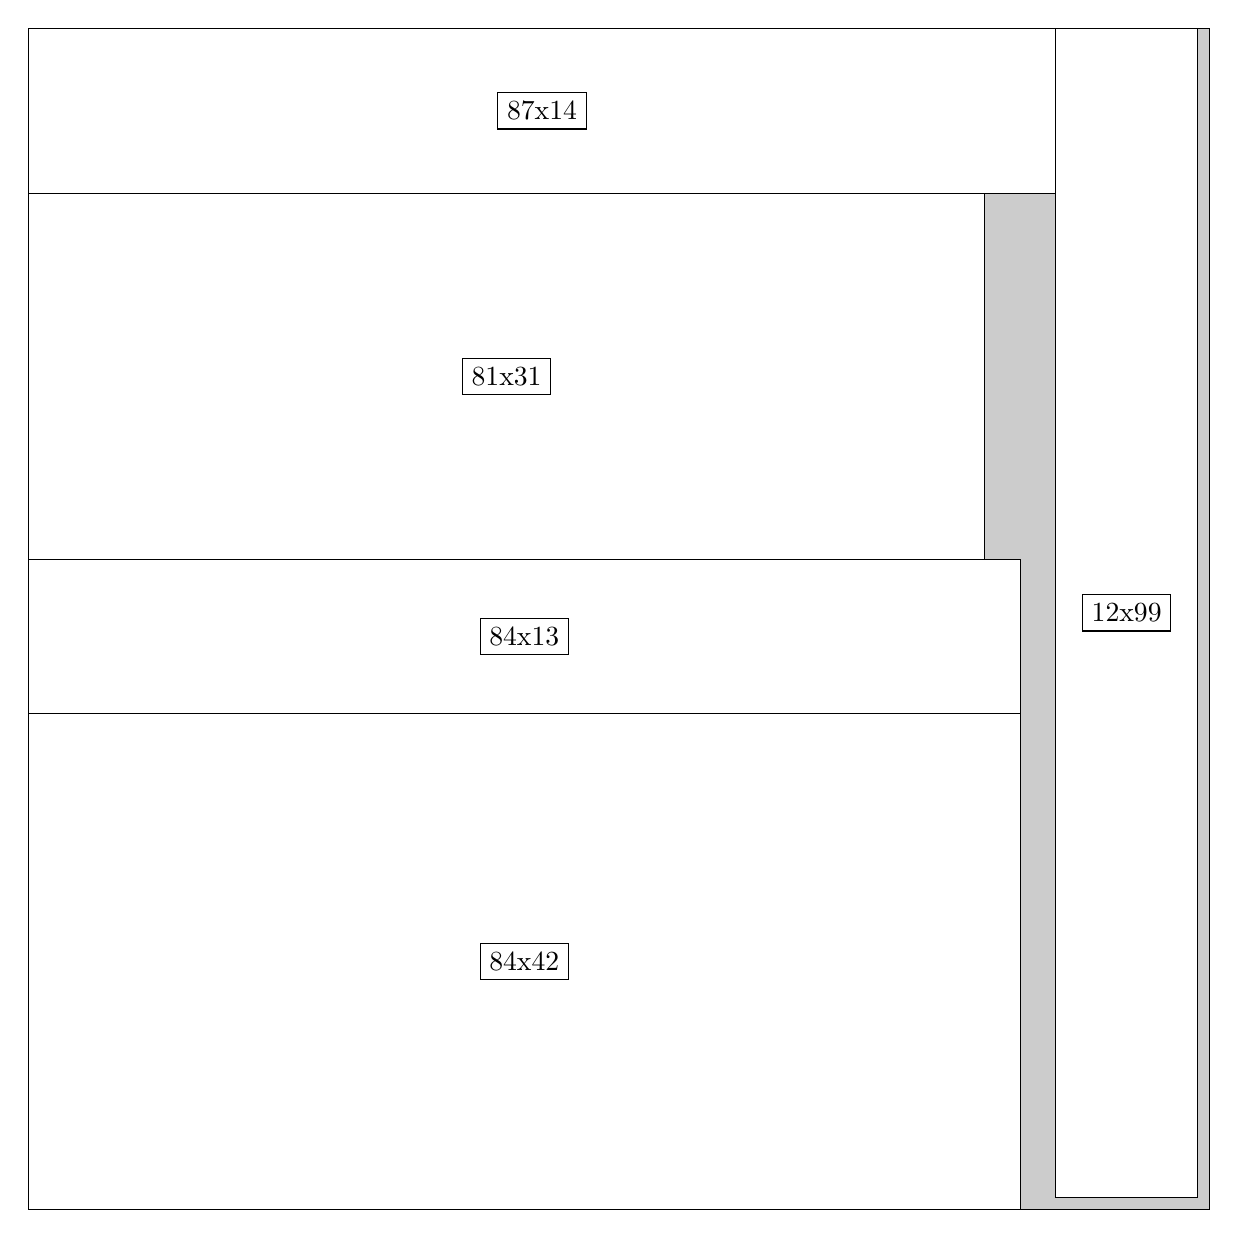
\begin{tikzpicture}[shorten >=1pt,scale=1.0,every node/.style={scale=1.0},->]
\tikzstyle{vertex}=[circle,fill=black!25,minimum size=14pt,inner sep=0pt]
\filldraw[fill=gray!40!white, draw=black] (0,0) rectangle (15.0,15.0);
\foreach \name/\x/\y/\w/\h in {84x42/0.0/0.0/12.6/6.3,81x31/0.0/8.25/12.15/4.6499999999999995,87x14/0.0/12.9/13.049999999999999/2.1,12x99/13.049999999999999/0.15/1.7999999999999998/14.85,84x13/0.0/6.3/12.6/1.95}
\filldraw[fill=white!40!white, draw=black] (\x,\y) rectangle node[draw] (\name) {\name} ++(\w,\h);
\end{tikzpicture}


w =84 , h =42 , x =0 , y =0 , v =3528
\par
w =81 , h =31 , x =0 , y =55 , v =2511
\par
w =87 , h =14 , x =0 , y =86 , v =1218
\par
w =12 , h =99 , x =87 , y =1 , v =1188
\par
w =84 , h =13 , x =0 , y =42 , v =1092
\par
\newpage


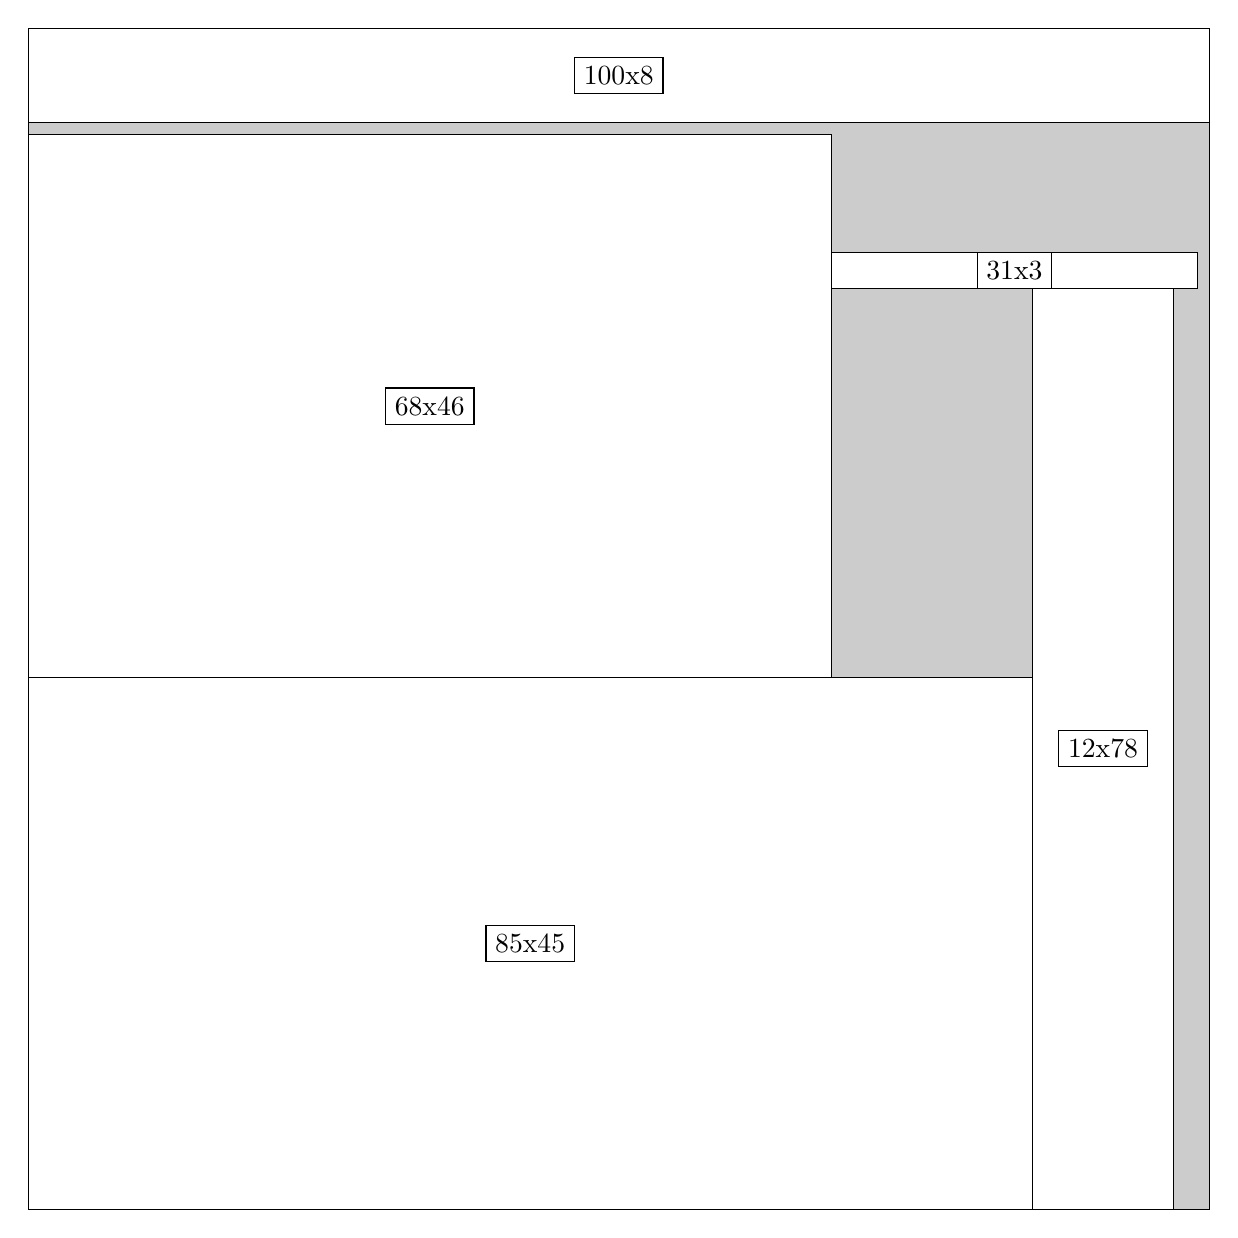
\begin{tikzpicture}[shorten >=1pt,scale=1.0,every node/.style={scale=1.0},->]
\tikzstyle{vertex}=[circle,fill=black!25,minimum size=14pt,inner sep=0pt]
\filldraw[fill=gray!40!white, draw=black] (0,0) rectangle (15.0,15.0);
\foreach \name/\x/\y/\w/\h in {85x45/0.0/0.0/12.75/6.75,68x46/0.0/6.75/10.2/6.8999999999999995,12x78/12.75/0.0/1.7999999999999998/11.7,100x8/0.0/13.799999999999999/15.0/1.2,31x3/10.2/11.7/4.6499999999999995/0.44999999999999996}
\filldraw[fill=white!40!white, draw=black] (\x,\y) rectangle node[draw] (\name) {\name} ++(\w,\h);
\end{tikzpicture}


w =85 , h =45 , x =0 , y =0 , v =3825
\par
w =68 , h =46 , x =0 , y =45 , v =3128
\par
w =12 , h =78 , x =85 , y =0 , v =936
\par
w =100 , h =8 , x =0 , y =92 , v =800
\par
w =31 , h =3 , x =68 , y =78 , v =93
\par
\newpage


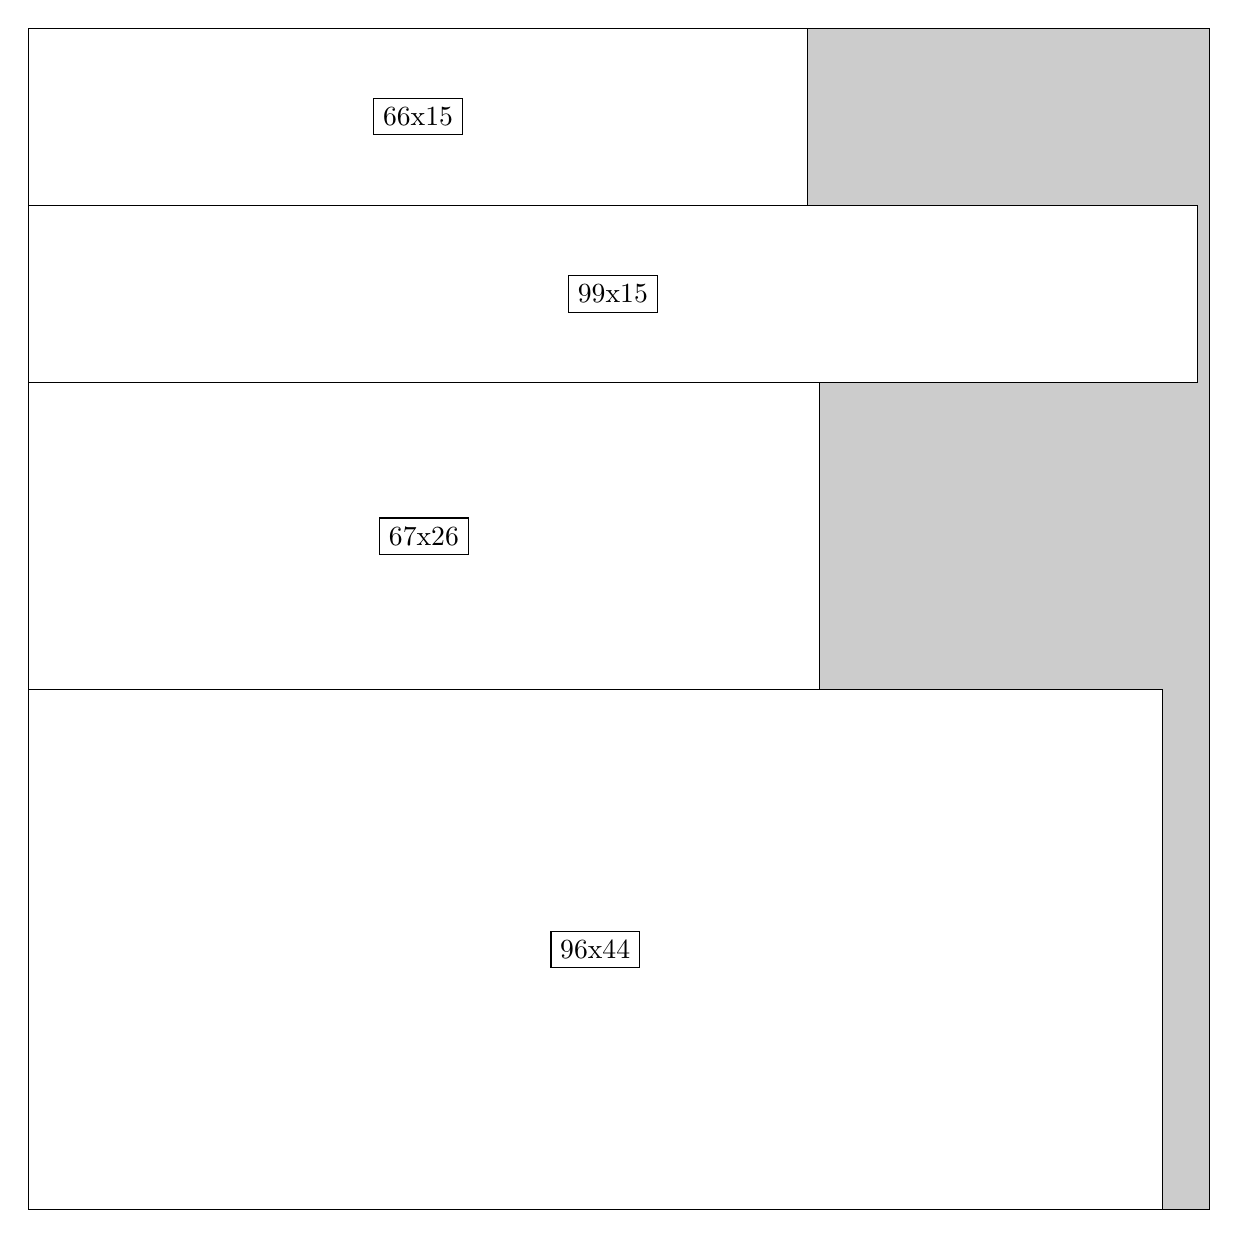
\begin{tikzpicture}[shorten >=1pt,scale=1.0,every node/.style={scale=1.0},->]
\tikzstyle{vertex}=[circle,fill=black!25,minimum size=14pt,inner sep=0pt]
\filldraw[fill=gray!40!white, draw=black] (0,0) rectangle (15.0,15.0);
\foreach \name/\x/\y/\w/\h in {96x44/0.0/0.0/14.399999999999999/6.6,67x26/0.0/6.6/10.049999999999999/3.9,99x15/0.0/10.5/14.85/2.25,66x15/0.0/12.75/9.9/2.25}
\filldraw[fill=white!40!white, draw=black] (\x,\y) rectangle node[draw] (\name) {\name} ++(\w,\h);
\end{tikzpicture}


w =96 , h =44 , x =0 , y =0 , v =4224
\par
w =67 , h =26 , x =0 , y =44 , v =1742
\par
w =99 , h =15 , x =0 , y =70 , v =1485
\par
w =66 , h =15 , x =0 , y =85 , v =990
\par
\newpage


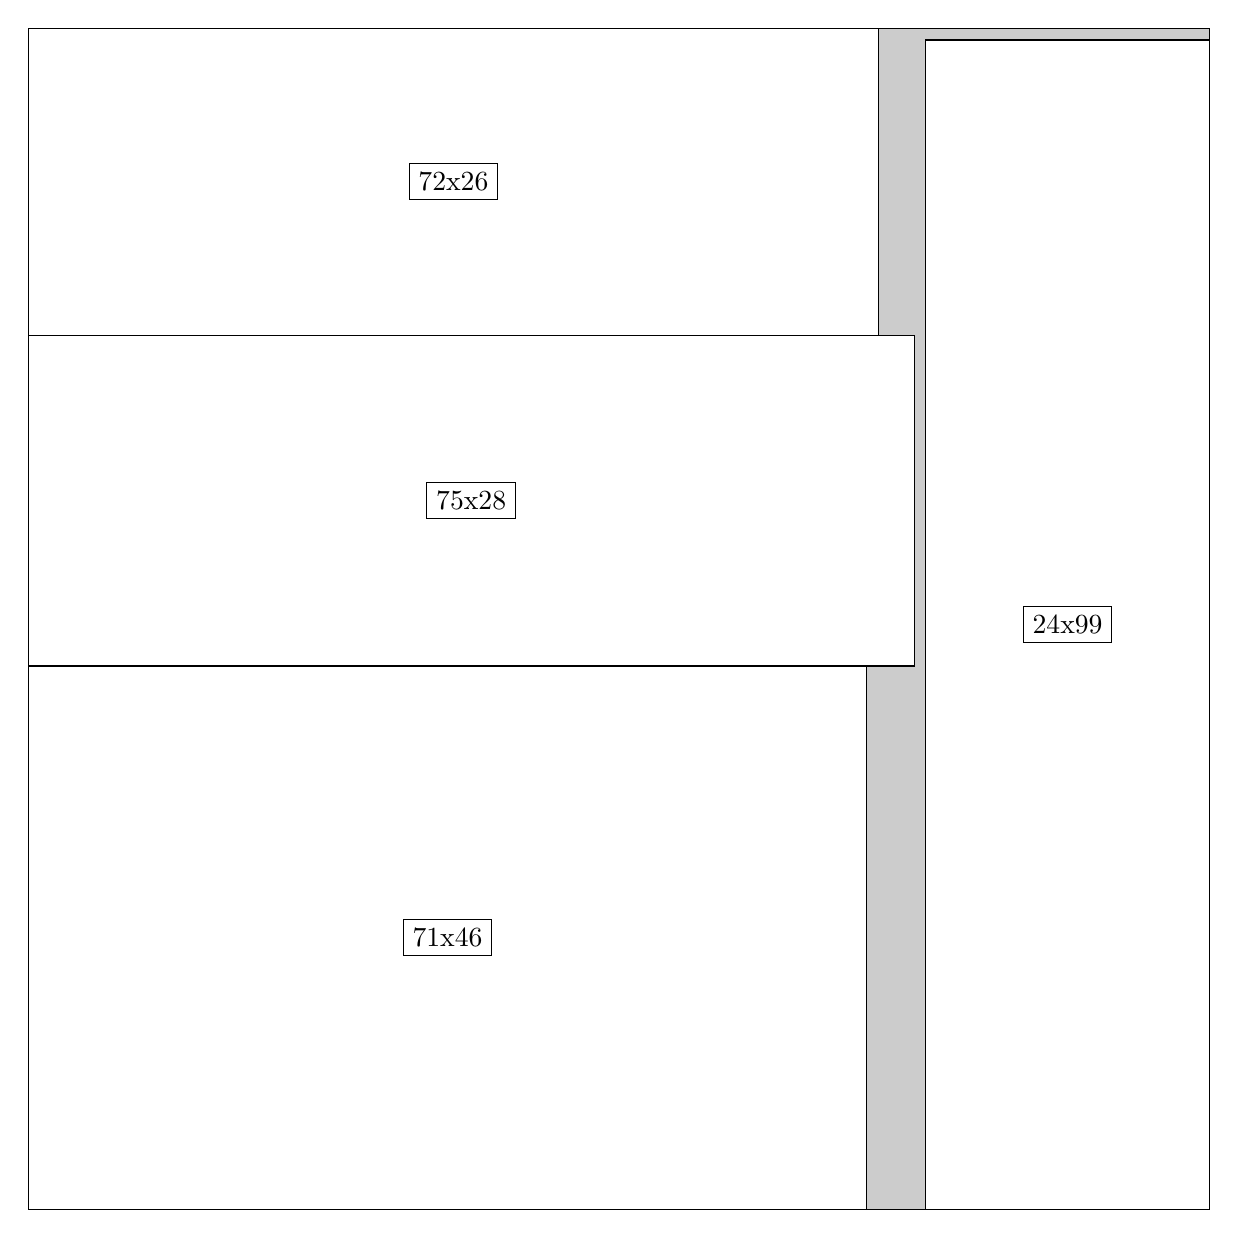
\begin{tikzpicture}[shorten >=1pt,scale=1.0,every node/.style={scale=1.0},->]
\tikzstyle{vertex}=[circle,fill=black!25,minimum size=14pt,inner sep=0pt]
\filldraw[fill=gray!40!white, draw=black] (0,0) rectangle (15.0,15.0);
\foreach \name/\x/\y/\w/\h in {71x46/0.0/0.0/10.65/6.8999999999999995,24x99/11.4/0.0/3.5999999999999996/14.85,75x28/0.0/6.8999999999999995/11.25/4.2,72x26/0.0/11.1/10.799999999999999/3.9}
\filldraw[fill=white!40!white, draw=black] (\x,\y) rectangle node[draw] (\name) {\name} ++(\w,\h);
\end{tikzpicture}


w =71 , h =46 , x =0 , y =0 , v =3266
\par
w =24 , h =99 , x =76 , y =0 , v =2376
\par
w =75 , h =28 , x =0 , y =46 , v =2100
\par
w =72 , h =26 , x =0 , y =74 , v =1872
\par
\newpage


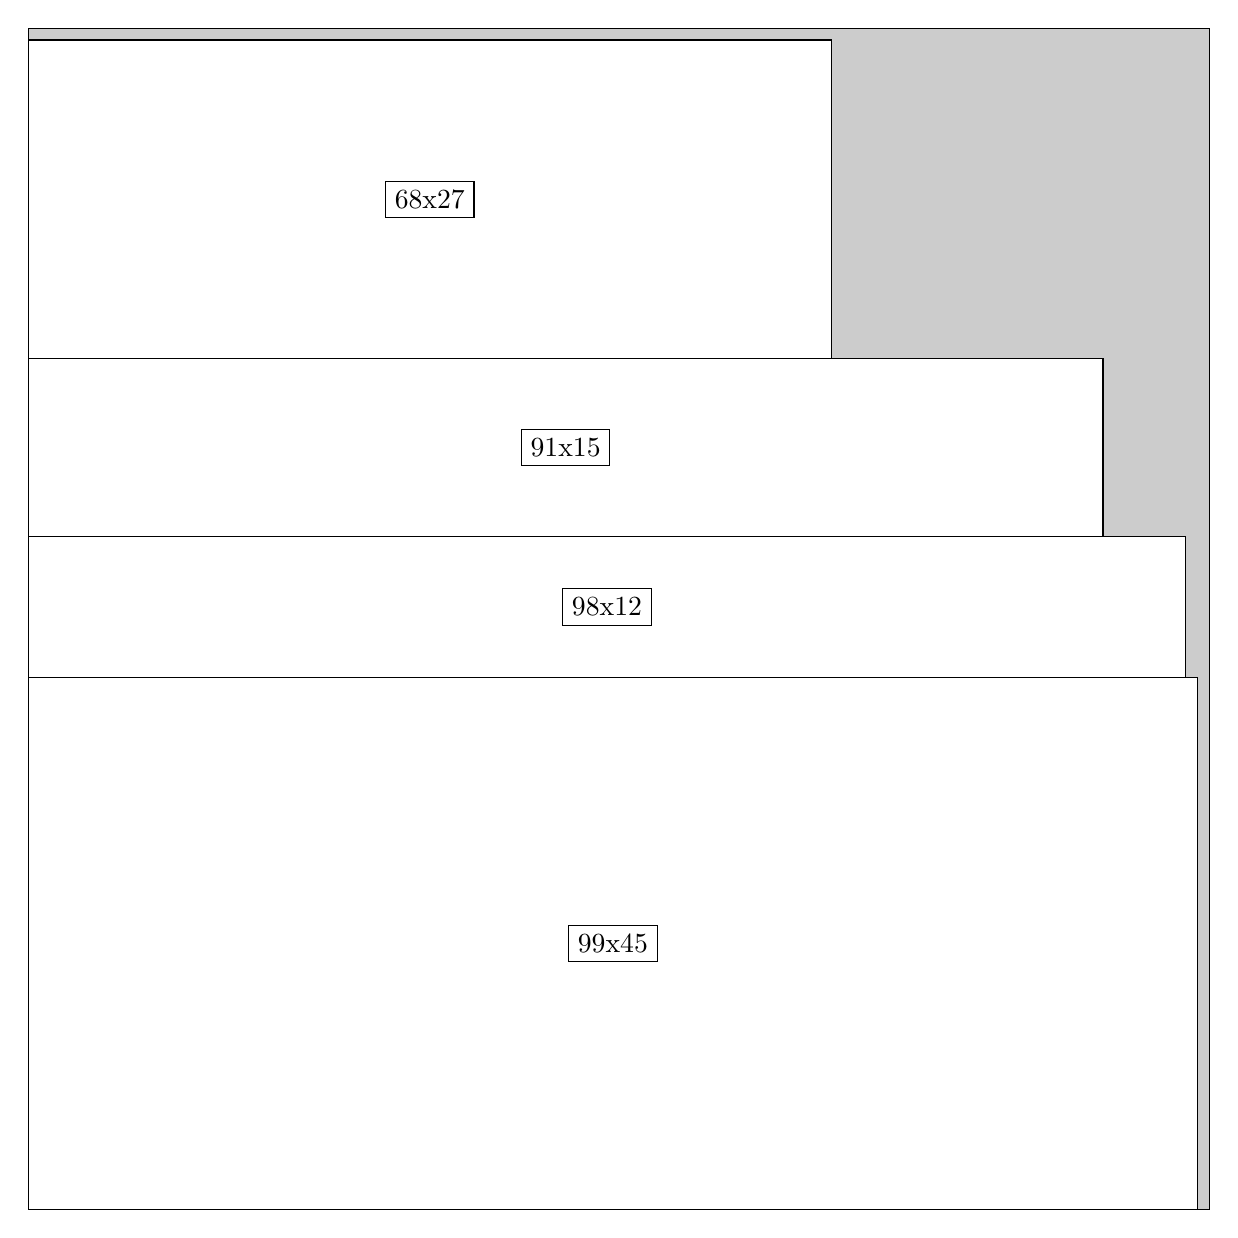
\begin{tikzpicture}[shorten >=1pt,scale=1.0,every node/.style={scale=1.0},->]
\tikzstyle{vertex}=[circle,fill=black!25,minimum size=14pt,inner sep=0pt]
\filldraw[fill=gray!40!white, draw=black] (0,0) rectangle (15.0,15.0);
\foreach \name/\x/\y/\w/\h in {99x45/0.0/0.0/14.85/6.75,68x27/0.0/10.799999999999999/10.2/4.05,91x15/0.0/8.549999999999999/13.65/2.25,98x12/0.0/6.75/14.7/1.7999999999999998}
\filldraw[fill=white!40!white, draw=black] (\x,\y) rectangle node[draw] (\name) {\name} ++(\w,\h);
\end{tikzpicture}


w =99 , h =45 , x =0 , y =0 , v =4455
\par
w =68 , h =27 , x =0 , y =72 , v =1836
\par
w =91 , h =15 , x =0 , y =57 , v =1365
\par
w =98 , h =12 , x =0 , y =45 , v =1176
\par
\newpage


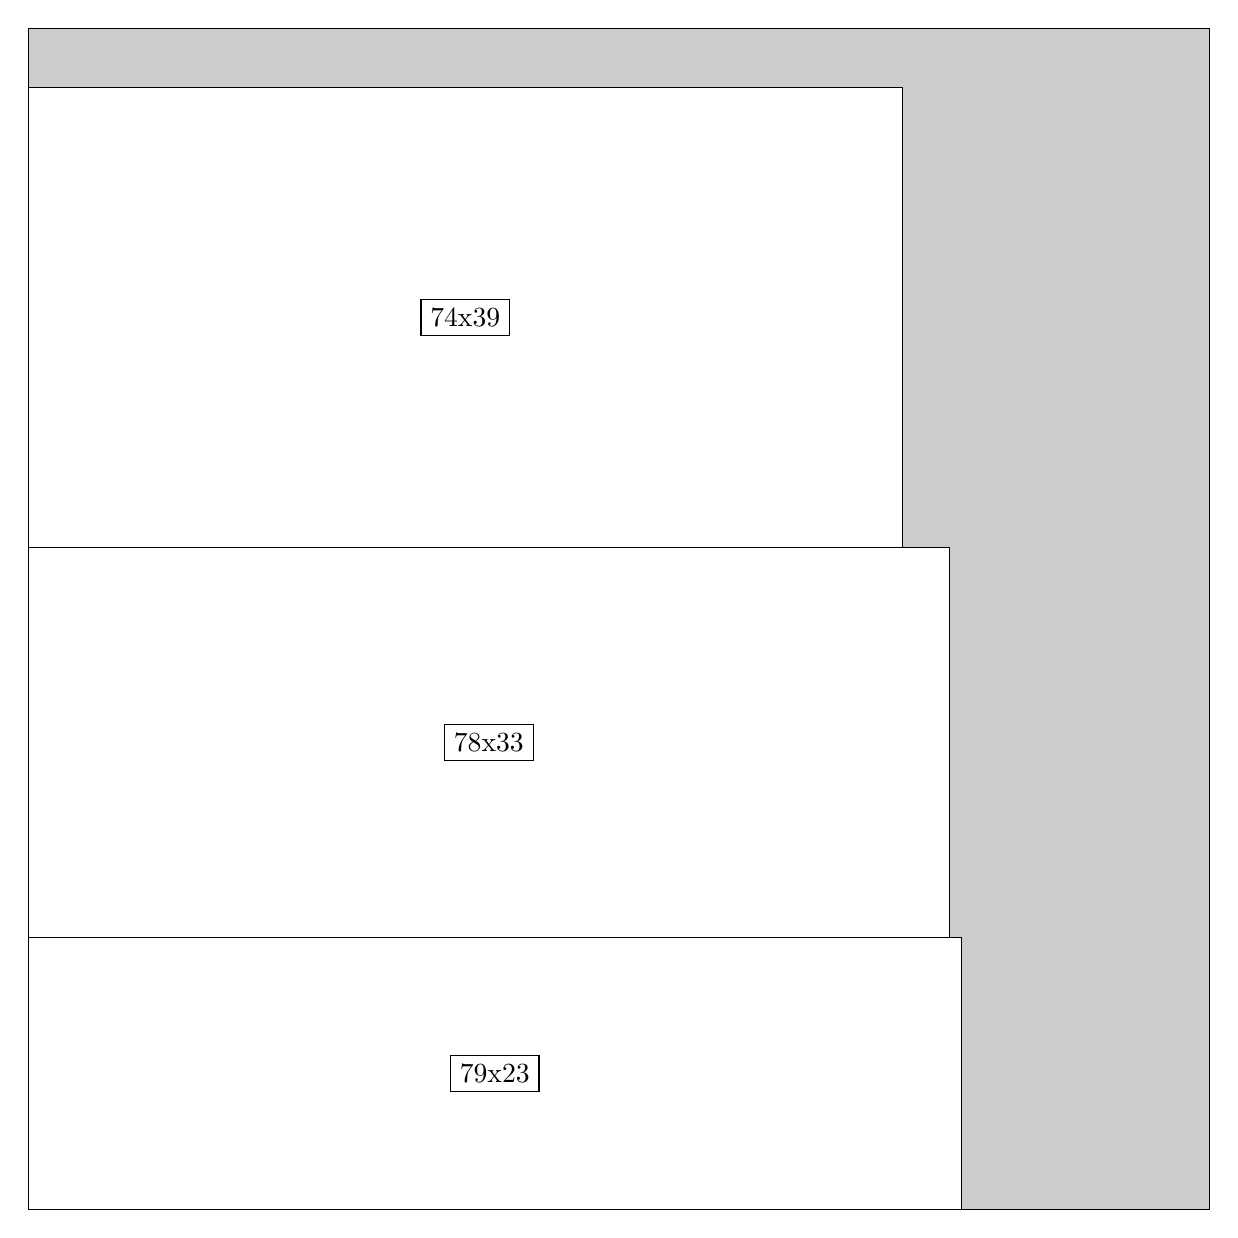
\begin{tikzpicture}[shorten >=1pt,scale=1.0,every node/.style={scale=1.0},->]
\tikzstyle{vertex}=[circle,fill=black!25,minimum size=14pt,inner sep=0pt]
\filldraw[fill=gray!40!white, draw=black] (0,0) rectangle (15.0,15.0);
\foreach \name/\x/\y/\w/\h in {74x39/0.0/8.4/11.1/5.85,78x33/0.0/3.4499999999999997/11.7/4.95,79x23/0.0/0.0/11.85/3.4499999999999997}
\filldraw[fill=white!40!white, draw=black] (\x,\y) rectangle node[draw] (\name) {\name} ++(\w,\h);
\end{tikzpicture}


w =74 , h =39 , x =0 , y =56 , v =2886
\par
w =78 , h =33 , x =0 , y =23 , v =2574
\par
w =79 , h =23 , x =0 , y =0 , v =1817
\par
\newpage


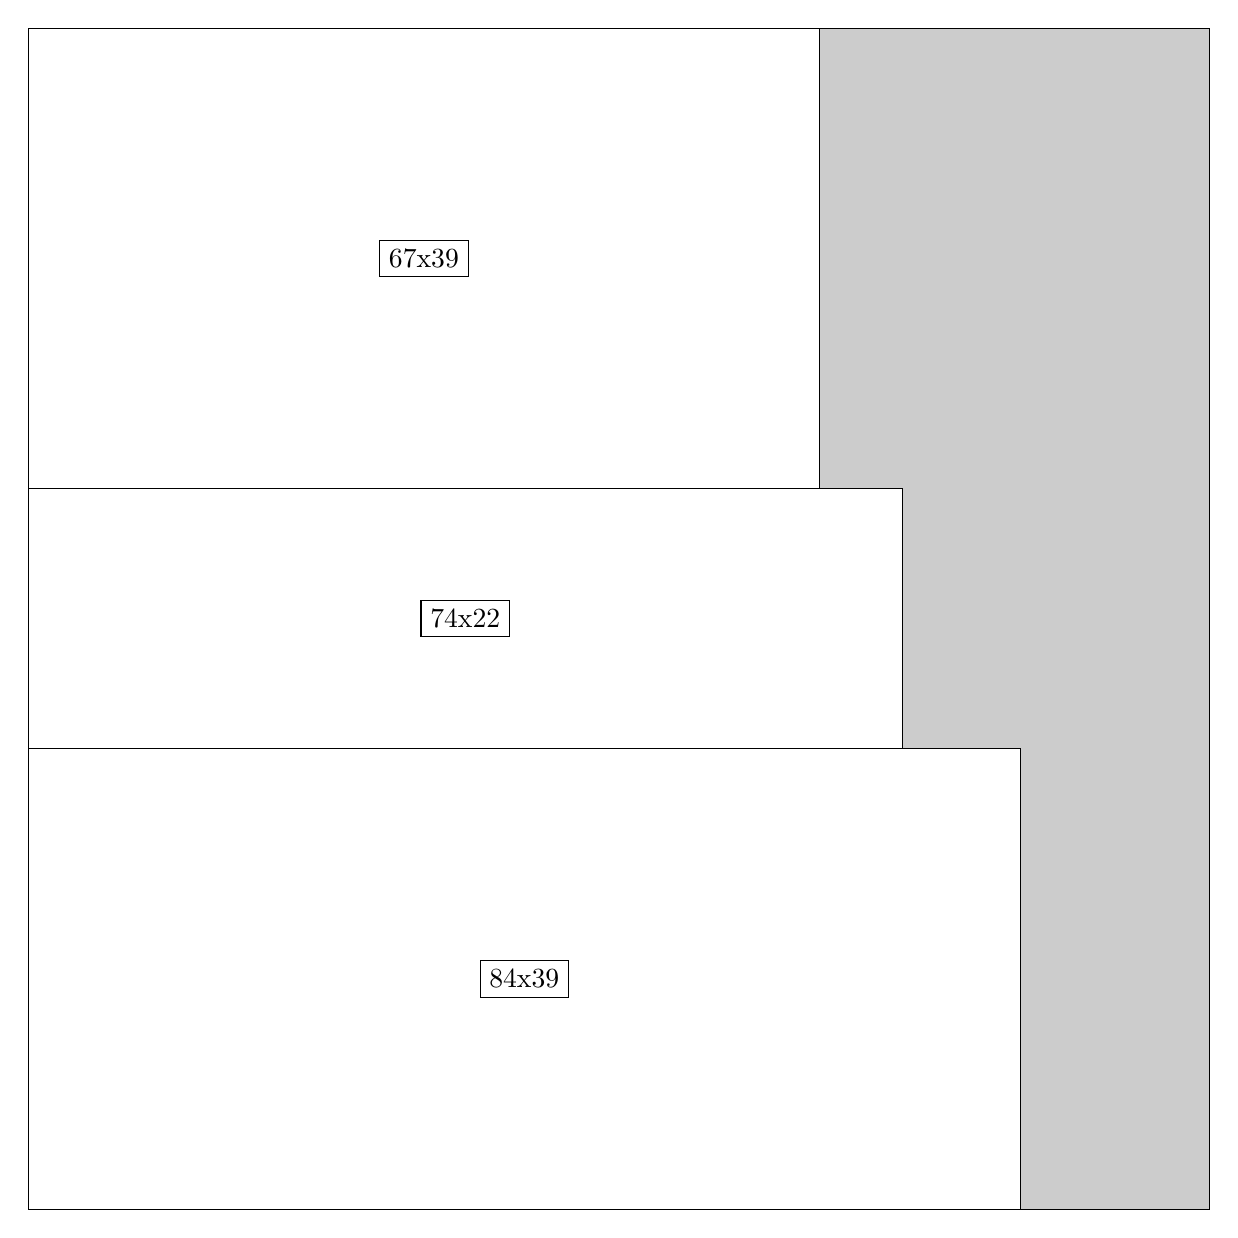
\begin{tikzpicture}[shorten >=1pt,scale=1.0,every node/.style={scale=1.0},->]
\tikzstyle{vertex}=[circle,fill=black!25,minimum size=14pt,inner sep=0pt]
\filldraw[fill=gray!40!white, draw=black] (0,0) rectangle (15.0,15.0);
\foreach \name/\x/\y/\w/\h in {84x39/0.0/0.0/12.6/5.85,67x39/0.0/9.15/10.049999999999999/5.85,74x22/0.0/5.85/11.1/3.3}
\filldraw[fill=white!40!white, draw=black] (\x,\y) rectangle node[draw] (\name) {\name} ++(\w,\h);
\end{tikzpicture}


w =84 , h =39 , x =0 , y =0 , v =3276
\par
w =67 , h =39 , x =0 , y =61 , v =2613
\par
w =74 , h =22 , x =0 , y =39 , v =1628
\par
\newpage


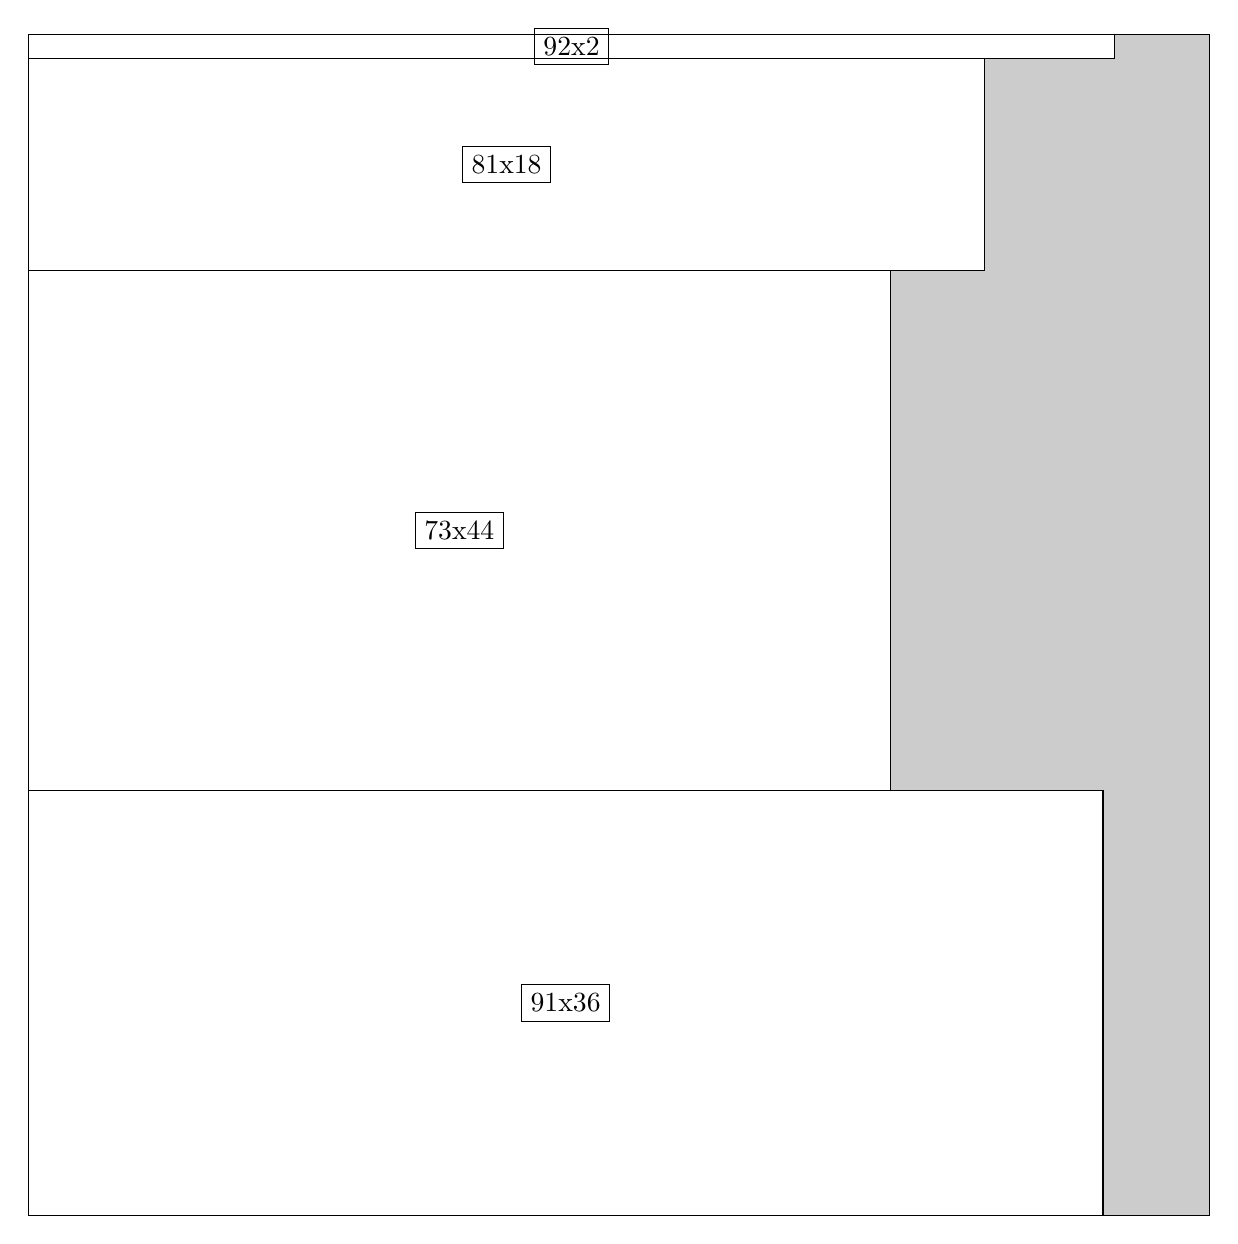
\begin{tikzpicture}[shorten >=1pt,scale=1.0,every node/.style={scale=1.0},->]
\tikzstyle{vertex}=[circle,fill=black!25,minimum size=14pt,inner sep=0pt]
\filldraw[fill=gray!40!white, draw=black] (0,0) rectangle (15.0,15.0);
\foreach \name/\x/\y/\w/\h in {91x36/0.0/0.0/13.65/5.3999999999999995,73x44/0.0/5.3999999999999995/10.95/6.6,81x18/0.0/12.0/12.15/2.6999999999999997,92x2/0.0/14.7/13.799999999999999/0.3}
\filldraw[fill=white!40!white, draw=black] (\x,\y) rectangle node[draw] (\name) {\name} ++(\w,\h);
\end{tikzpicture}


w =91 , h =36 , x =0 , y =0 , v =3276
\par
w =73 , h =44 , x =0 , y =36 , v =3212
\par
w =81 , h =18 , x =0 , y =80 , v =1458
\par
w =92 , h =2 , x =0 , y =98 , v =184
\par
\newpage


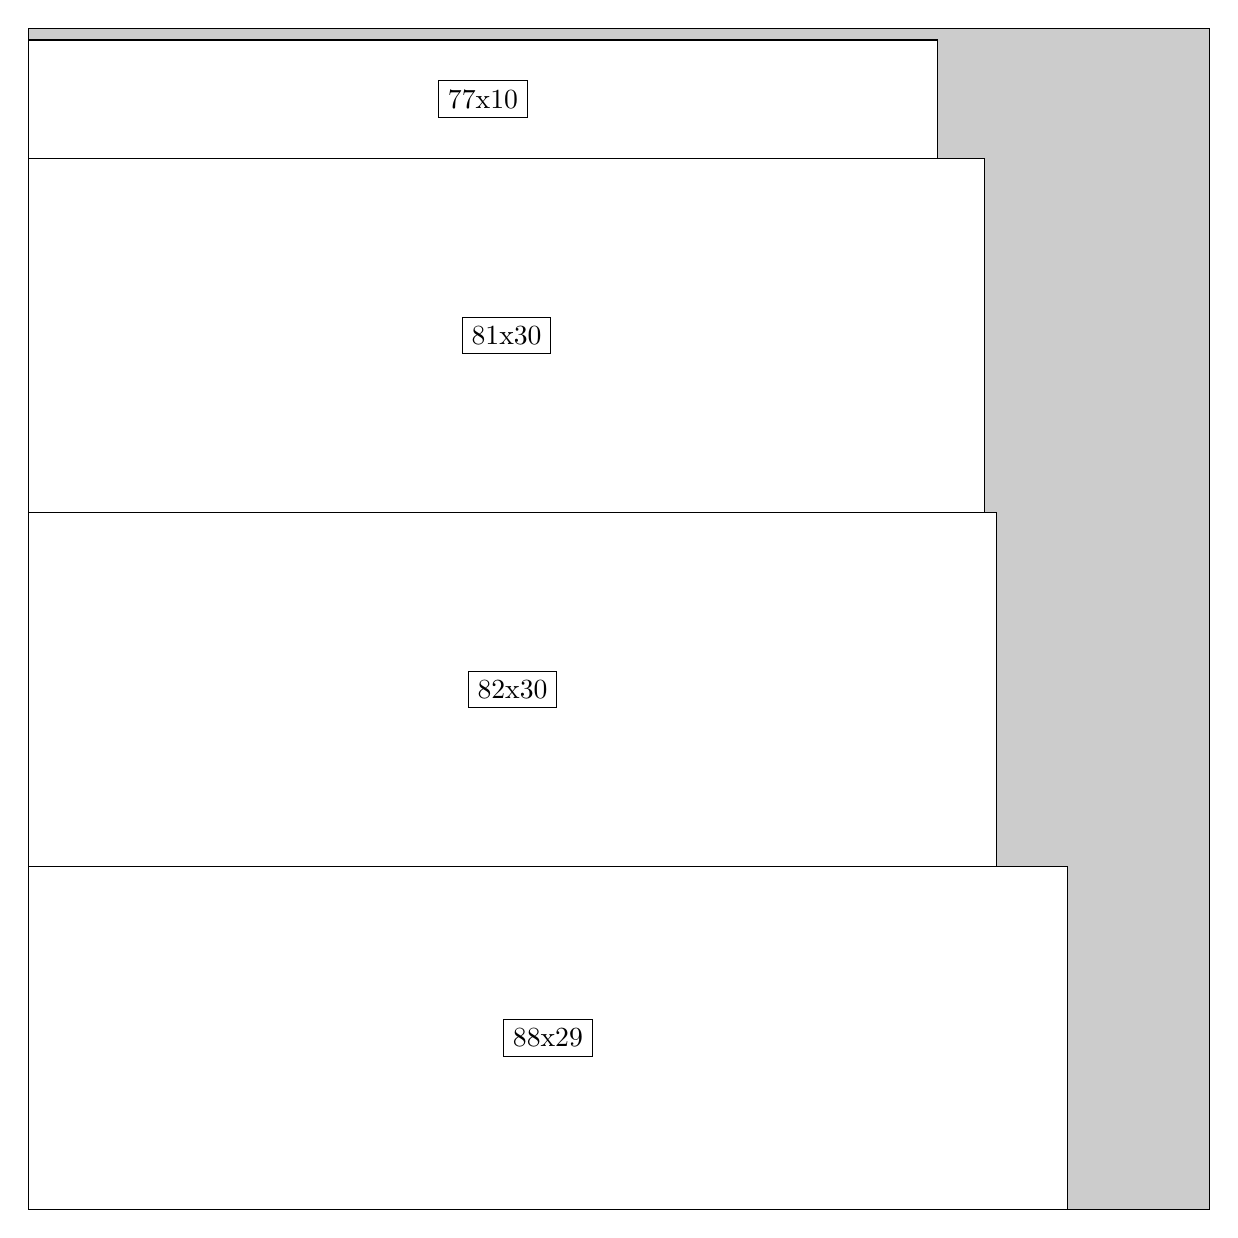
\begin{tikzpicture}[shorten >=1pt,scale=1.0,every node/.style={scale=1.0},->]
\tikzstyle{vertex}=[circle,fill=black!25,minimum size=14pt,inner sep=0pt]
\filldraw[fill=gray!40!white, draw=black] (0,0) rectangle (15.0,15.0);
\foreach \name/\x/\y/\w/\h in {88x29/0.0/0.0/13.2/4.35,82x30/0.0/4.35/12.299999999999999/4.5,81x30/0.0/8.85/12.15/4.5,77x10/0.0/13.35/11.549999999999999/1.5}
\filldraw[fill=white!40!white, draw=black] (\x,\y) rectangle node[draw] (\name) {\name} ++(\w,\h);
\end{tikzpicture}


w =88 , h =29 , x =0 , y =0 , v =2552
\par
w =82 , h =30 , x =0 , y =29 , v =2460
\par
w =81 , h =30 , x =0 , y =59 , v =2430
\par
w =77 , h =10 , x =0 , y =89 , v =770
\par
\newpage


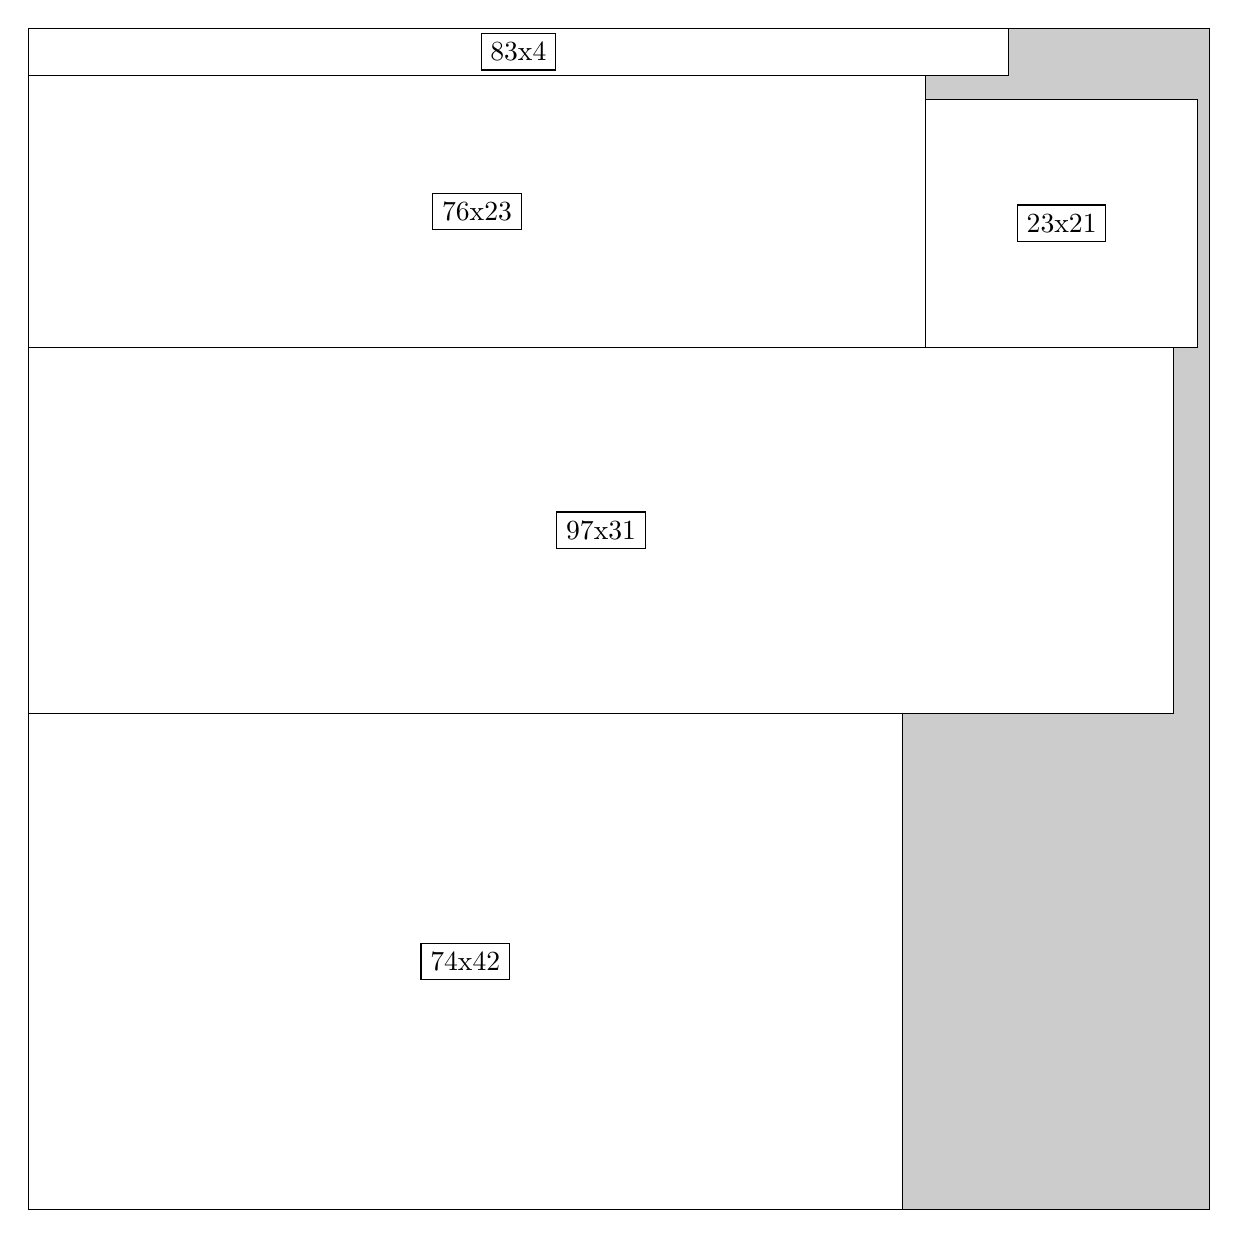
\begin{tikzpicture}[shorten >=1pt,scale=1.0,every node/.style={scale=1.0},->]
\tikzstyle{vertex}=[circle,fill=black!25,minimum size=14pt,inner sep=0pt]
\filldraw[fill=gray!40!white, draw=black] (0,0) rectangle (15.0,15.0);
\foreach \name/\x/\y/\w/\h in {74x42/0.0/0.0/11.1/6.3,97x31/0.0/6.3/14.549999999999999/4.6499999999999995,76x23/0.0/10.95/11.4/3.4499999999999997,23x21/11.4/10.95/3.4499999999999997/3.15,83x4/0.0/14.399999999999999/12.45/0.6}
\filldraw[fill=white!40!white, draw=black] (\x,\y) rectangle node[draw] (\name) {\name} ++(\w,\h);
\end{tikzpicture}


w =74 , h =42 , x =0 , y =0 , v =3108
\par
w =97 , h =31 , x =0 , y =42 , v =3007
\par
w =76 , h =23 , x =0 , y =73 , v =1748
\par
w =23 , h =21 , x =76 , y =73 , v =483
\par
w =83 , h =4 , x =0 , y =96 , v =332
\par
\newpage


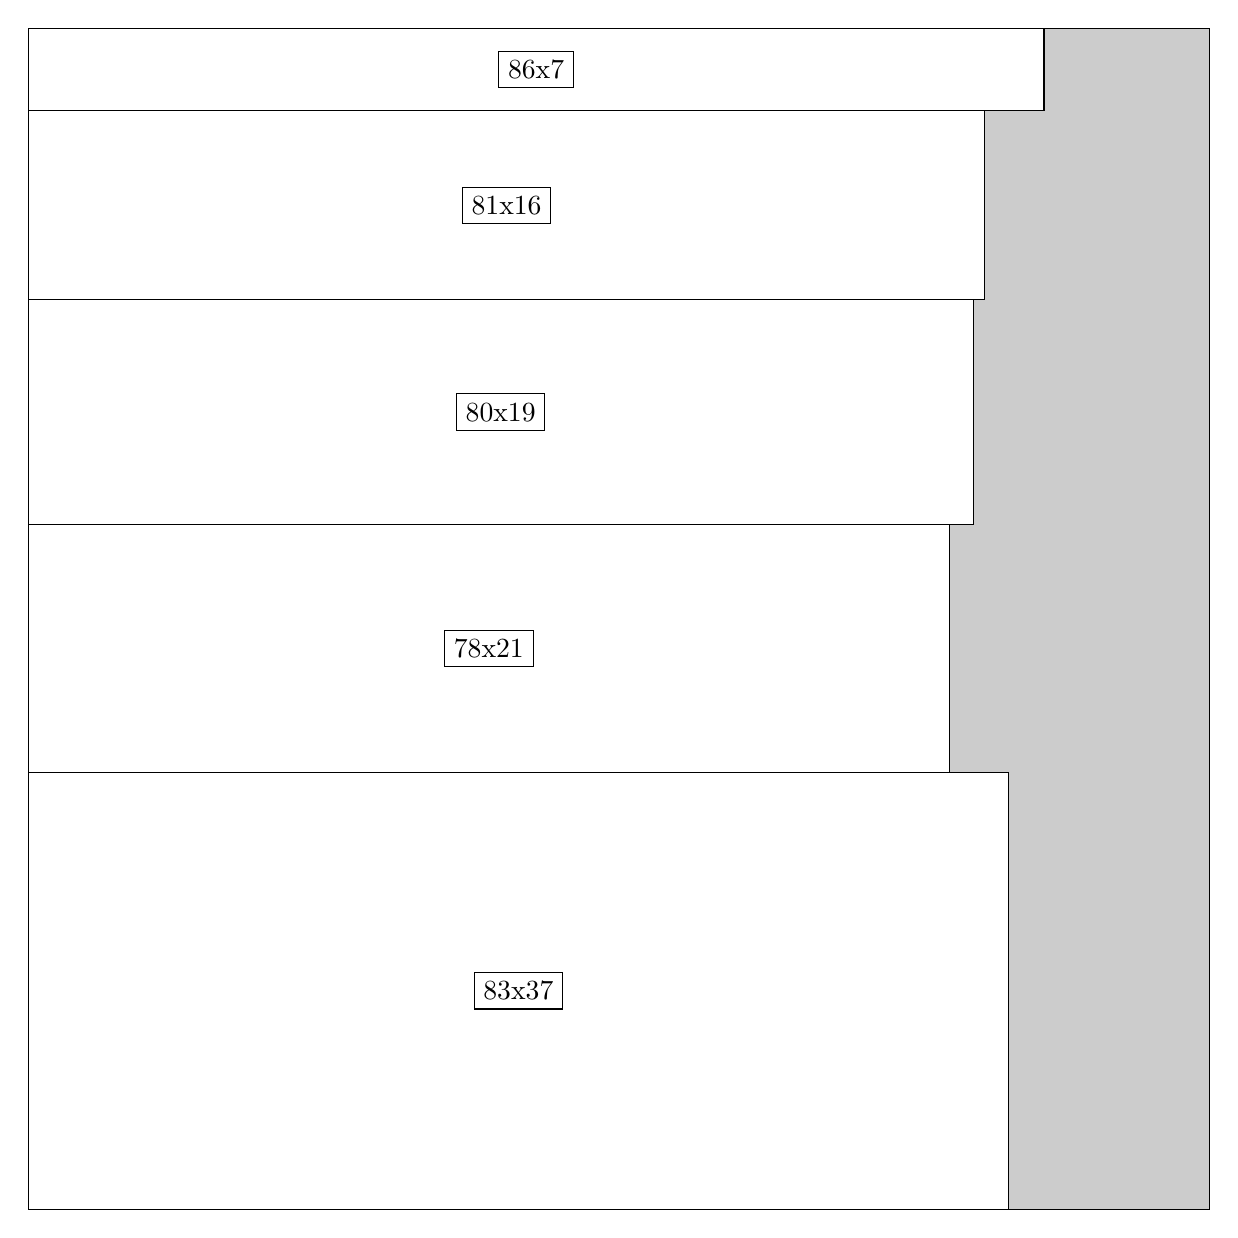
\begin{tikzpicture}[shorten >=1pt,scale=1.0,every node/.style={scale=1.0},->]
\tikzstyle{vertex}=[circle,fill=black!25,minimum size=14pt,inner sep=0pt]
\filldraw[fill=gray!40!white, draw=black] (0,0) rectangle (15.0,15.0);
\foreach \name/\x/\y/\w/\h in {83x37/0.0/0.0/12.45/5.55,78x21/0.0/5.55/11.7/3.15,80x19/0.0/8.7/12.0/2.85,81x16/0.0/11.549999999999999/12.15/2.4,86x7/0.0/13.95/12.9/1.05}
\filldraw[fill=white!40!white, draw=black] (\x,\y) rectangle node[draw] (\name) {\name} ++(\w,\h);
\end{tikzpicture}


w =83 , h =37 , x =0 , y =0 , v =3071
\par
w =78 , h =21 , x =0 , y =37 , v =1638
\par
w =80 , h =19 , x =0 , y =58 , v =1520
\par
w =81 , h =16 , x =0 , y =77 , v =1296
\par
w =86 , h =7 , x =0 , y =93 , v =602
\par
\newpage


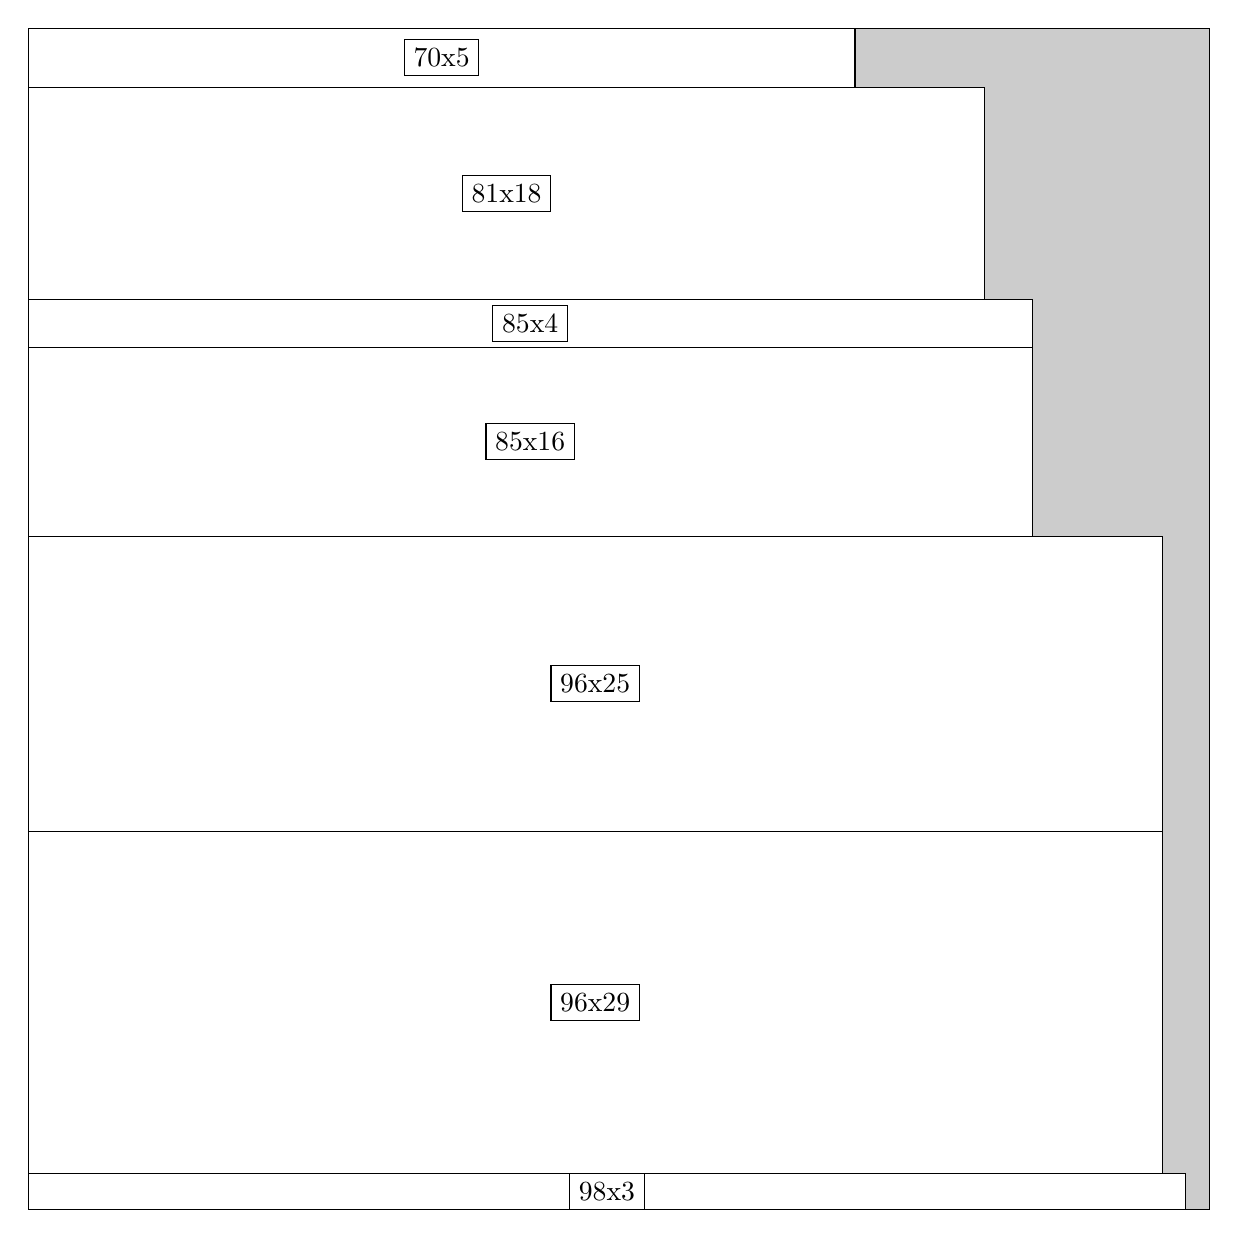
\begin{tikzpicture}[shorten >=1pt,scale=1.0,every node/.style={scale=1.0},->]
\tikzstyle{vertex}=[circle,fill=black!25,minimum size=14pt,inner sep=0pt]
\filldraw[fill=gray!40!white, draw=black] (0,0) rectangle (15.0,15.0);
\foreach \name/\x/\y/\w/\h in {96x29/0.0/0.44999999999999996/14.399999999999999/4.35,96x25/0.0/4.8/14.399999999999999/3.75,81x18/0.0/11.549999999999999/12.15/2.6999999999999997,85x16/0.0/8.549999999999999/12.75/2.4,70x5/0.0/14.25/10.5/0.75,85x4/0.0/10.95/12.75/0.6,98x3/0.0/0.0/14.7/0.44999999999999996}
\filldraw[fill=white!40!white, draw=black] (\x,\y) rectangle node[draw] (\name) {\name} ++(\w,\h);
\end{tikzpicture}


w =96 , h =29 , x =0 , y =3 , v =2784
\par
w =96 , h =25 , x =0 , y =32 , v =2400
\par
w =81 , h =18 , x =0 , y =77 , v =1458
\par
w =85 , h =16 , x =0 , y =57 , v =1360
\par
w =70 , h =5 , x =0 , y =95 , v =350
\par
w =85 , h =4 , x =0 , y =73 , v =340
\par
w =98 , h =3 , x =0 , y =0 , v =294
\par
\newpage


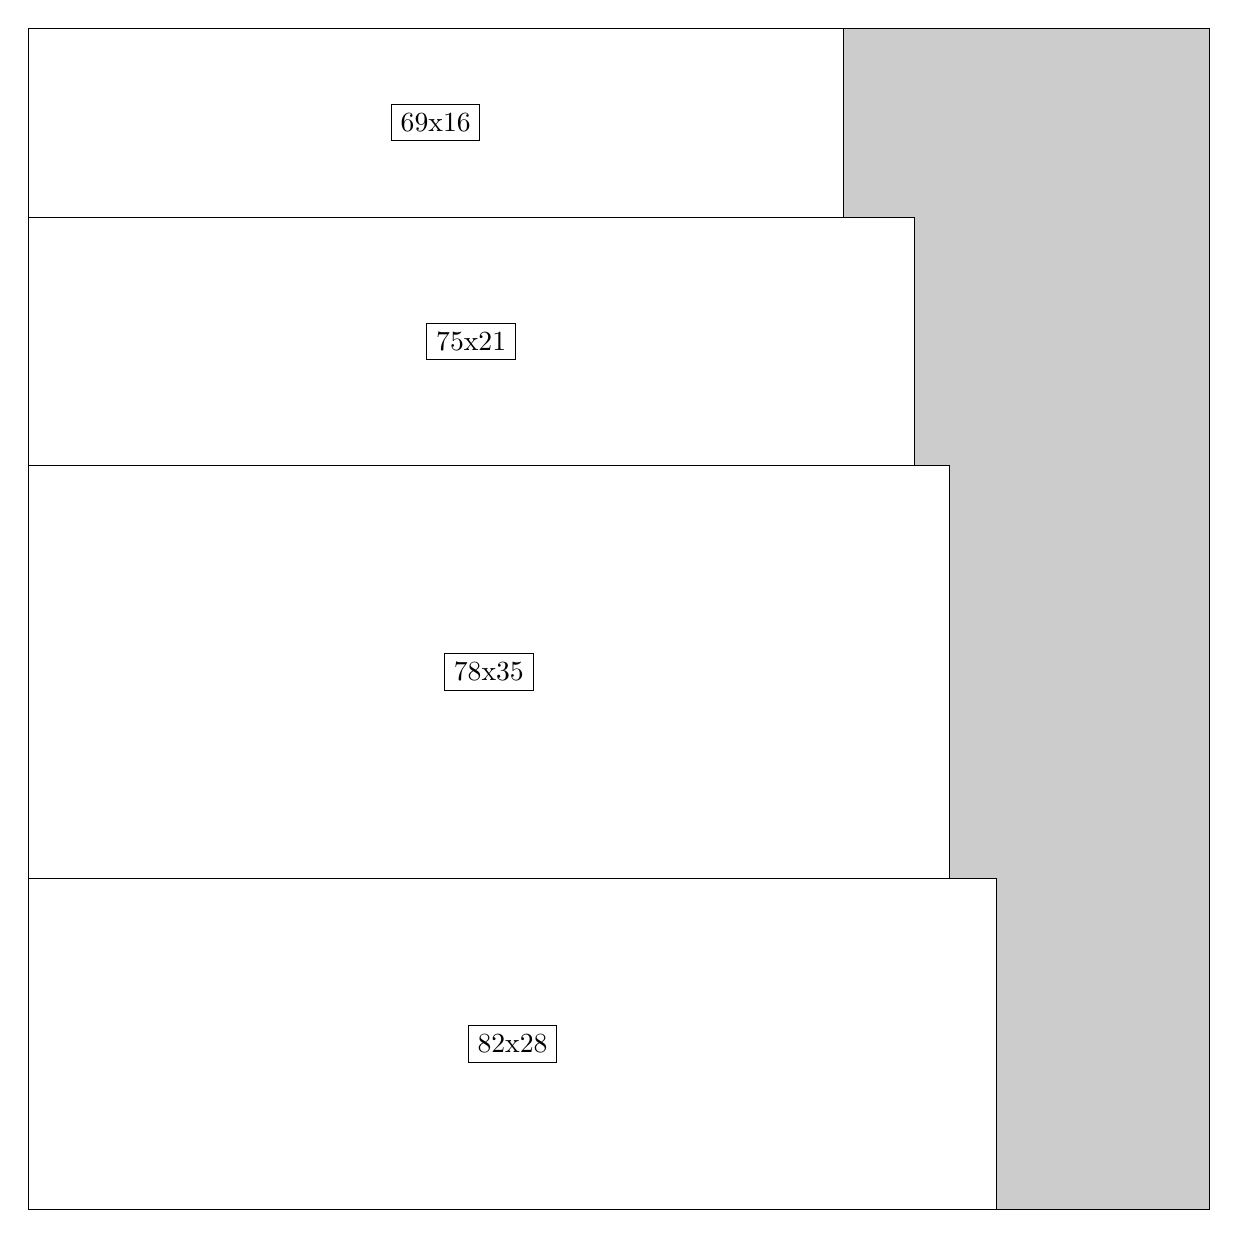
\begin{tikzpicture}[shorten >=1pt,scale=1.0,every node/.style={scale=1.0},->]
\tikzstyle{vertex}=[circle,fill=black!25,minimum size=14pt,inner sep=0pt]
\filldraw[fill=gray!40!white, draw=black] (0,0) rectangle (15.0,15.0);
\foreach \name/\x/\y/\w/\h in {78x35/0.0/4.2/11.7/5.25,82x28/0.0/0.0/12.299999999999999/4.2,75x21/0.0/9.45/11.25/3.15,69x16/0.0/12.6/10.35/2.4}
\filldraw[fill=white!40!white, draw=black] (\x,\y) rectangle node[draw] (\name) {\name} ++(\w,\h);
\end{tikzpicture}


w =78 , h =35 , x =0 , y =28 , v =2730
\par
w =82 , h =28 , x =0 , y =0 , v =2296
\par
w =75 , h =21 , x =0 , y =63 , v =1575
\par
w =69 , h =16 , x =0 , y =84 , v =1104
\par
\newpage


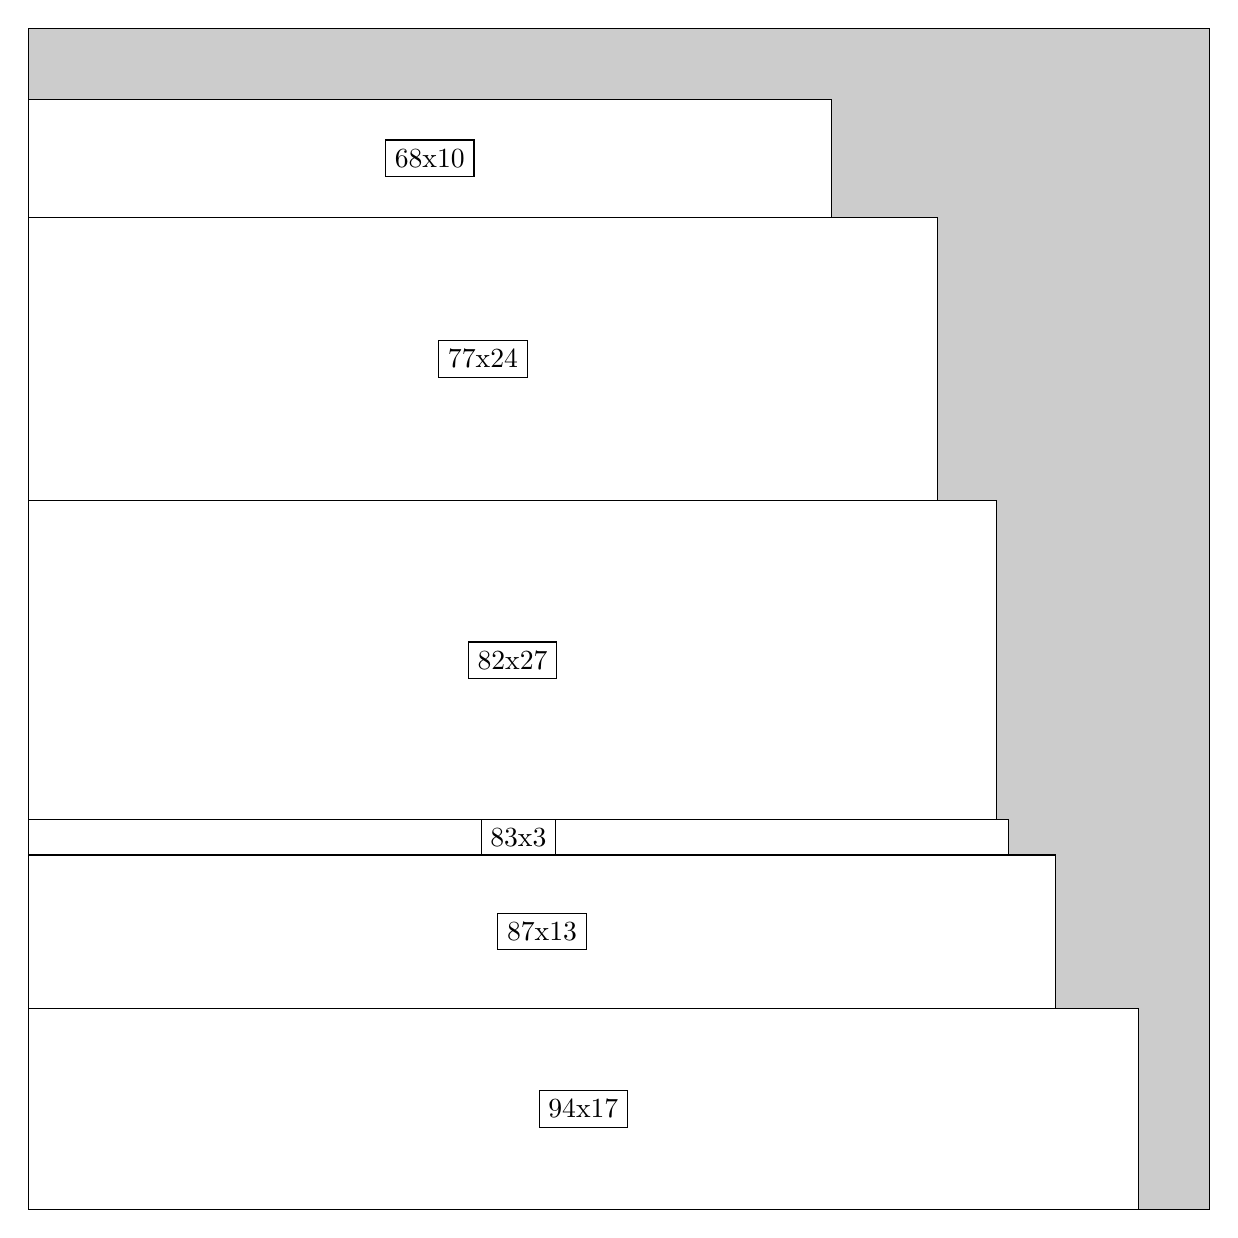
\begin{tikzpicture}[shorten >=1pt,scale=1.0,every node/.style={scale=1.0},->]
\tikzstyle{vertex}=[circle,fill=black!25,minimum size=14pt,inner sep=0pt]
\filldraw[fill=gray!40!white, draw=black] (0,0) rectangle (15.0,15.0);
\foreach \name/\x/\y/\w/\h in {82x27/0.0/4.95/12.299999999999999/4.05,87x13/0.0/2.55/13.049999999999999/1.95,94x17/0.0/0.0/14.1/2.55,77x24/0.0/9.0/11.549999999999999/3.5999999999999996,68x10/0.0/12.6/10.2/1.5,83x3/0.0/4.5/12.45/0.44999999999999996}
\filldraw[fill=white!40!white, draw=black] (\x,\y) rectangle node[draw] (\name) {\name} ++(\w,\h);
\end{tikzpicture}


w =82 , h =27 , x =0 , y =33 , v =2214
\par
w =87 , h =13 , x =0 , y =17 , v =1131
\par
w =94 , h =17 , x =0 , y =0 , v =1598
\par
w =77 , h =24 , x =0 , y =60 , v =1848
\par
w =68 , h =10 , x =0 , y =84 , v =680
\par
w =83 , h =3 , x =0 , y =30 , v =249
\par
\newpage


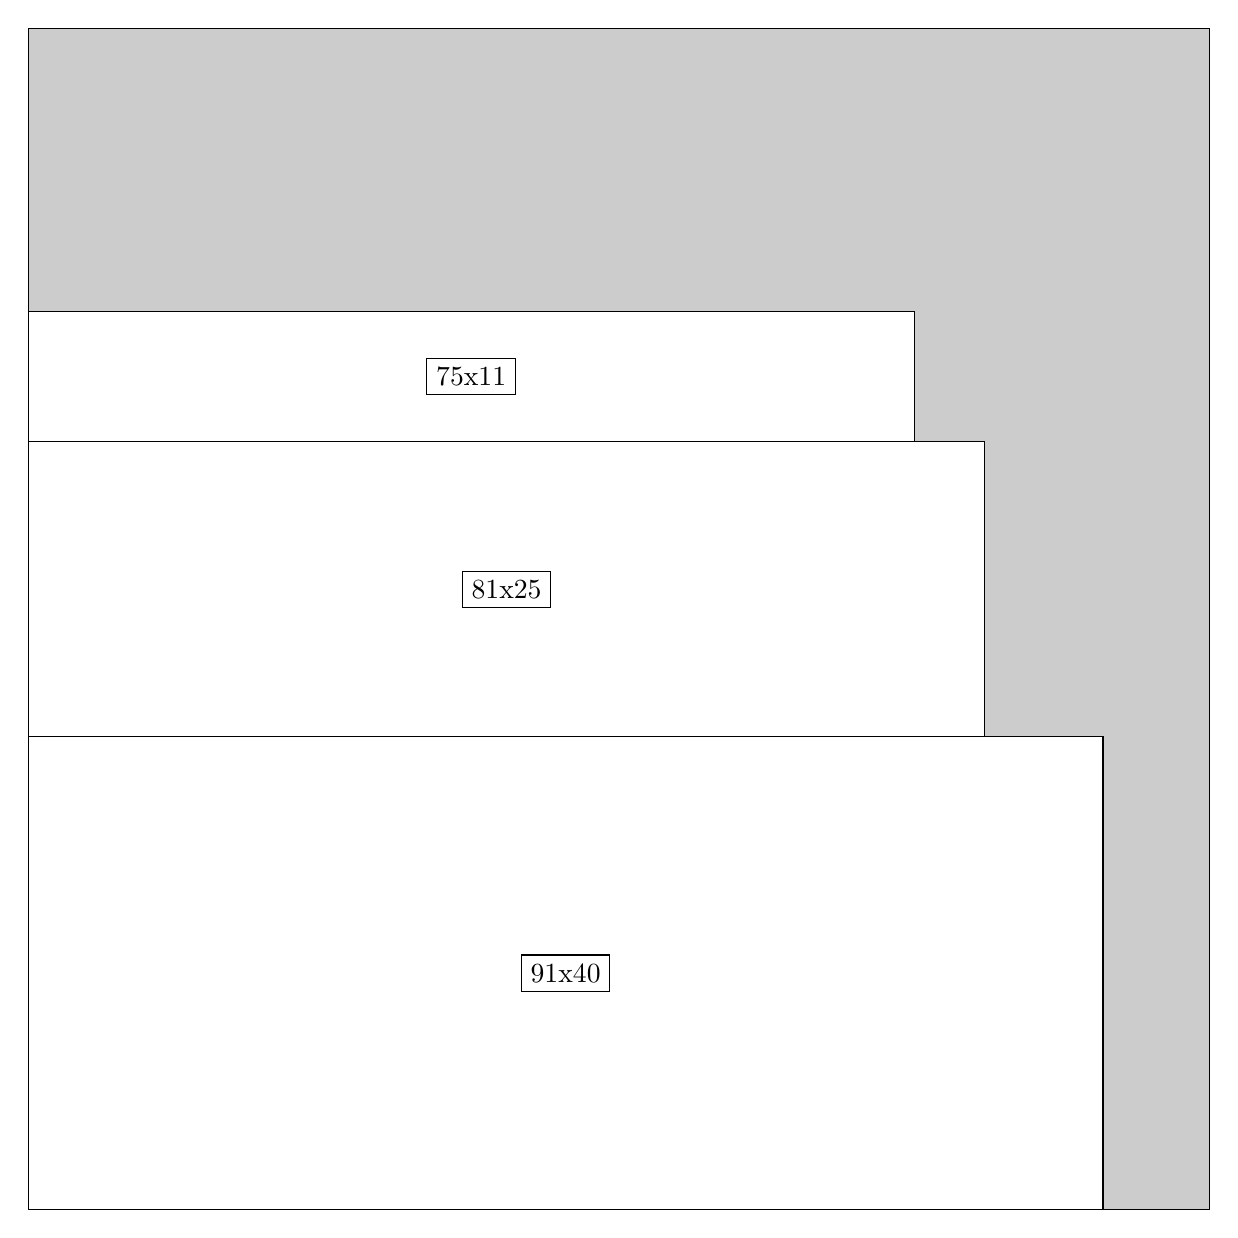
\begin{tikzpicture}[shorten >=1pt,scale=1.0,every node/.style={scale=1.0},->]
\tikzstyle{vertex}=[circle,fill=black!25,minimum size=14pt,inner sep=0pt]
\filldraw[fill=gray!40!white, draw=black] (0,0) rectangle (15.0,15.0);
\foreach \name/\x/\y/\w/\h in {91x40/0.0/0.0/13.65/6.0,81x25/0.0/6.0/12.15/3.75,75x11/0.0/9.75/11.25/1.65}
\filldraw[fill=white!40!white, draw=black] (\x,\y) rectangle node[draw] (\name) {\name} ++(\w,\h);
\end{tikzpicture}


w =91 , h =40 , x =0 , y =0 , v =3640
\par
w =81 , h =25 , x =0 , y =40 , v =2025
\par
w =75 , h =11 , x =0 , y =65 , v =825
\par
\newpage


\end{document}